\documentclass[12pt, %
openright, 
oneside, %
%twoside, %TCC: Se seu texto tem mais de 100 páginas, descomente esta linha e comente a anterior
a4paper,    %
%english,   %
brazil]{facom-ufu-abntex2}

\makeatletter
\setlength{\@fptop}{0pt}
\makeatother

\usepackage{graphicx}
\graphicspath{{figuras/}{pictures/}{images/}{./}} % where to search for the images

\newcommand{\blue}[1]{\textcolor{blue}{#1}}
\newcommand{\red}[1]{\textcolor{red}{#1}}


\autor{Luis Felipe Costa Fernandes de Menezes} %TCC
\data{2026}
\orientador{Pedro Augusto Queiroz de Assis} %TCC
%\coorientador{Algum?} %TCC

% ---
% Informações de dados para CAPA e FOLHA DE ROSTO
% ---

\titulo{Emprego de visão computacional para identificação de
comportamento suspeito no varejo} %TCC

\hypersetup{pdfkeywords={visão computacional}{varejo}{furto}{deep learning}{análise de vídeo}} %TCC

\begin{document} 
\frenchspacing 

% ----------------------------------------------------------
% ELEMENTOS PRÉ-TEXTUAIS
% ----------------------------------------------------------
%\pretextual
\imprimircapa
\imprimirfolhaderosto


% ---
% Inserir folha de aprovação
% ---
%
% \includepdf{folhadeaprovacao_final.pdf} %TCC: depois de aprovado o trabalho, descomente esta linha e comente o próximo bloco para incluir scan da folha de aprovação.
%
\begin{folhadeaprovacao}

  \begin{center}
    {\ABNTEXchapterfont\large\imprimirautor}

    \vspace*{\fill}\vspace*{\fill}
    {\ABNTEXchapterfont\bfseries\Large\imprimirtitulo}
    \vspace*{\fill}
    
    \hspace{.45\textwidth}
    \begin{minipage}{.5\textwidth}
        \imprimirpreambulo
    \end{minipage}%
    \vspace*{\fill}
   \end{center}
    
   Trabalho aprovado. \imprimirlocal, XX de XX de 2026: %TCC:

   \assinatura{\textbf{\imprimirorientador} \\ Orientador}  
   \assinatura{\textbf{Professor}}% \\ Convidado 1} %TCC:
   \assinatura{\textbf{Professor}}% \\ Convidado 2} %TCC:
   %\assinatura{\textbf{Professor} \\ Convidado 3}
   %\assinatura{\textbf{Professor} \\ Convidado 4}
      
   \begin{center}
    \vspace*{0.5cm}
    {\large\imprimirlocal}
    \par
    {\large\imprimirdata}
    \vspace*{1cm}
  \end{center}
  
\end{folhadeaprovacao}
% ---


%%As seções dedicatória, agradecimento e epígrafe não são obrigatórias.
%%Só as mantenha se achar pertinente.

% ---
% Dedicatória
% ---
%\begin{dedicatoria}
%   \vspace*{\fill}
%   \centering
%   \noindent
%   \textit{Dedico a \lipsum[10]}  %TCC:
%   \vspace*{\fill}
%\end{dedicatoria}
% ---

% ---
% Agradecimentos
% ---
%\begin{agradecimentos}
%Agradeço a \lipsum[30]. %TCC:
%\end{agradecimentos}
% ---

% ---
% Epígrafe
% ---
%\begin{epigrafe}
%    \vspace*{\fill}
%	\begin{flushright}
%		\textit{``Alguma citação que ache conveniente? \lipsum[10]''} %TCC:
%	\end{flushright}
%\end{epigrafe}
% ---



\begin{resumo} %TCC:
 % Segundo a \citeonline[3.1-3.2]{NBR6028:2003}, o resumo deve ressaltar o
 % objetivo, o método, os resultados e as conclusões do documento. A ordem e a extensão
 % destes itens dependem do tipo de resumo (informativo ou indicativo) e do
 % tratamento que cada item recebe no documento original. O resumo deve ser
 % precedido da referência do documento, com exceção do resumo inserido no
 % próprio documento. (\ldots) As palavras-chave devem figurar logo abaixo do
 % resumo, antecedidas da expressão Palavras-chave:, separadas entre si por
 % ponto e finalizadas também por ponto.

 \vspace{\onelineskip}
    
 \noindent
 % \textbf{Palavras-chave}: Até, cinco, palavras-chave, separadas, por, vírgulas. %TCC:
\end{resumo}

% ---
% inserir lista de ilustrações
% ---
\pdfbookmark[0]{\listfigurename}{lof}
\listoffigures*
\cleardoublepage
% ---

% ---
% inserir lista de tabelas
% ---
\pdfbookmark[0]{\listtablename}{lot}
\listoftables*
\cleardoublepage
% ---



% ---
% inserir lista de abreviaturas e siglas
% ---
\begin{siglas} %TCC:
\item[CFTV] Circuito Fechado de Televisão
\item[IA] Inteligência Artificial
\item[RNC] Rede Neural Convolucional
\item[GPU] Graphics Processing Unit
\item[ViT] Vision Transformer
\item[ML] Machine Learning
\item[DL] Deep Learning
\item[SL] Supervised Learning
\item[RGB] Red, Green, Blue
\item[I3D] Inflated 3D ConvNet
\item[K400] Kinetics-400
\item[SSv2] Something-Something V2
\item[BCE] Binary Cross-Entropy
\item[CEL] Cross-Entropy Loss
\item[AUC-ROC] Area Under the Receiver Operating Characteristic Curve
\item [FPS] Frames Per Second
\item [Adam] Adaptive Moment Estimation
\item [AdamW] Adam with Decoupled Weight Decay
\end{siglas}
% ---

%% ---
%% inserir lista de símbolos, se for adequado ao trabalho. %TCC:
%% ---
%\begin{simbolos}
%  \item[$ \Gamma $] Letra grega Gama
%  \item[$ \Lambda $] Lambda
%  \item[$ \zeta $] Letra grega minúscula zeta
%  \item[$ \in $] Pertence
%\end{simbolos}
%% ---

% ---
% inserir o sumario
% ---
\pdfbookmark[0]{\contentsname}{toc}
\tableofcontents*
\cleardoublepage
% ---





% ----------------------------------------------------------
% ELEMENTOS TEXTUAIS
% ----------------------------------------------------------
\textual


% ----------------------------------------------------------
% Introdução
% ----------------------------------------------------------

\chapter[Introdução]{Introdução}
O setor varejista global enfrenta um desafio crônico que diminui suas margens de lucro e afeta a sustentabilidade de suas operações: as perdas de inventário por furto. O alto fluxo de indivíduos em ambientes comerciais de livre acesso cria um ecossistema suscetível a esse tipo de conduta. Em escala global, a National Retail Federation reportou um aumento de 93\% nos incidentes de furtos em 2024 em relação aos níveis de 2019, resultando em perdas financeiras anuais que ultrapassam dezenas de bilhões de dólares e forçando as empresas a repensarem ativamente suas estratégias de segurança \cite{nrf}. No contexto nacional, ações ilícitas geram impactos de tal magnitude nas receitas das empresas do setor que em 2023 foi observado um aumento de 27\%, em relação ao ano anterior, no número de empresas que possuem áreas dedicadas à prevenção de perdas, totalizando 95\% de todas as empresas analisadas \cite{abrappe2024}.

As áreas dedicadas à prevenção de perdas atuam no monitoramento e mitigação de diferentes fontes de prejuízo, incluindo quebras operacionais, furtos externos, furtos internos, erros de inventário e fraudes. Em particular, os furtos configuram-se como a segunda maior causa de perdas no varejo, correspondendo a aproximadamente 31\% dos R\$34,9 bilhões em prejuízos registrados no ano analisado \cite{abrappe2024}, justificando investimentos maciços em segurança. Nesse sentido, agentes de vigilância constituem um componente essencial na proteção do setor varejista, sendo que uma parcela significativa dos investimentos em prevenção de perdas é direcionada a esses funcionários \cite{efforts}.

Entretanto, métodos tradicionais de vigilância e proteção de ativos têm se mostrado insuficientes. A dependência quase exclusiva de Circuitos Fechados de Televisão (CFTV) operados de forma manual exige que os agentes de monitoramento mantenham atenção constante e ininterrupta a dezenas de monitores simultaneamente, o que pode resultar em cegueira por desatenção \cite{gorila}. Estudos empíricos conduzidos especificamente em ambientes de monitoramento demonstram que operadores humanos, independentemente de possuírem treinamento prévio para tarefa, chegam a falhar na detecção de até 66\% dos eventos críticos que ocorrem claramente em seus campos de visão \cite{blind}. Na prática operacional, essa limitação inerente ao fator humano se traduz em taxas significativamente reduzidas de detecção de comportamentos ilícitos em tempo real. É exatamente neste ponto que a visão computacional e o aprendizado de máquina assumem o protagonismo, oferecendo soluções automatizadas capazes de monitorar o espaço físico, reconhecer padrões complexos com precisão e sinalizar comportamentos anômalos antes que o suposto infrator abandone o estabelecimento.

Sob a perspectiva da inovação, transformar a infraestrutura legada e passiva de CFTV em uma rede de sensores ativos, impulsionados por Inteligência Artificial (IA), pode representar um salto imenso na eficiência do monitoramento. Contudo, a transição da simples aquisição de imagens bidimensionais para a compreensão semântica profunda do comportamento de indivíduos por meio da análise do vídeo configura um problema extremamente complexo na área de visão computacional. Ao contrário do reconhecimento clássico de imagens estáticas, que depende da extração de características espaciais puras, como formas geométricas e detecção de bordas, a análise comportamental em vídeo exige a modelagem indispensável do espectro temporal. Abordagens puramente espaciais mostram-se insuficientes nesse contexto, sobretudo na distinção de ações quirais\footnote{Movimentos temporalmente opostos, como abrir versus fechar uma porta.}, uma vez que não capturam a evolução temporal das interações na cena \cite{quiral}. Consequentemente, comportamentos suspeitos de furto no varejo não podem ser adequadamente caracterizados a partir da análise isolada de quadros individuais.

A literatura voltada para a análise de vídeos, especialmente na detecção automatizada de anomalias, tem sido objeto de uma vigorosa e incessante exploração ao longo das últimas décadas. Com a disponibilidade de um poder computacional cada vez maior utilizando múltiplas GPUs, as metodologias de análise de vídeo transitaram de abordagens baseadas em heurísticas manuais para arquiteturas de aprendizado profundo ricas em representação semântica. Em particular, o problema da detecção de furtos tem sido solucionado por meio de diferentes métodos. Abordagens clássicas utilizam subtração de fundo para segmentar objetos em movimento do fundo estático da cena, seguidos de operações morfológicas para extrair \textit{bounding boxes} e analisar variações espaciais ao longo do tempo \cite{Rahangdale,azevedo}. Entretanto, essas abordagens mostraram baixa robustez em ambientes reais devido à sensibilidade a mudanças de iluminação, oclusões e à incapacidade de capturar o contexto semântico.

Já os métodos baseados em IA/aprendizado profundo passaram a empregar, dentre outras metodologias, Redes Neurais Convolucionais 3D (RNCs 3D), capazes de modelar simultaneamente informações espaciais e temporais. Nesse tipo de modelo de IA, se aprende a atribuir maiores pontuações de anomalia aos trechos mais suspeitos mesmo sem anotações precisas do instante em que o evento ocorre \cite{sultani}. No entanto, o treinamento inicial de RNCs 3D é extremamente custoso, exigindo a criação de bancos de dados relativamente extensos, como o UCF-Crime \cite{sultani}, que consiste em longos vídeos de vigilância não editados que abrangem 13 tipos de ocorrências do mundo real, incluindo furto em lojas, com mais de 128 horas.

A fim de contornar essa explosão de parâmetros e dados exigida pelas RNCs 3D, surgiram as Redes Neurais Híbridas, nas quais o processo analítico de aprendizado é decomposto em duas etapas sequenciais e distintas: redes convolucionais bidimensionais tradicionais pré-treinadas para extração de características espaciais dos quadros combinadas com redes recorrentes responsáveis por modelar as dependências temporais das sequências de vídeo \cite{muneer}. Embora apresentem bom equilíbrio entre desempenho e custo computacional, esses métodos podem perder informações espaciais detalhadas, pois a dinâmica temporal é analisada apenas após a compressão das características visuais extraídas pela RNC.

Paralelamente, surgiram abordagens orientadas à preservação de privacidade, nas quais algoritmos de estimativa de pose extraem apenas os pontos-chave do corpo humano, convertendo os movimentos dos indivíduos em representações esqueléticas anonimizadas. A dinâmica dessas articulações é então modelada por Redes Convolucionais de Grafos Espaço-Temporais \cite{poselift}, capazes de analisar padrões biomecânicos de movimento para identificar comportamentos suspeitos. Como desvantagem dessa abordagem, tem-se uma redução da eficácia na presença de oclusões, o que frequentemente ocorre em ambientes de varejo.

Por fim, a vertente que tem dominado as pesquisas contemporâneas explora a maturação e evolução dos Transformadores de Visão (\textit{Vision Transformers}), que adapta a tecnologia originalmente desenvolvida para decodificar linguagem natural para o escopo temporal do vídeo, nos quais sequências de quadros são divididas em \textit{patches} visuais e processadas por mecanismos de auto-atenção capazes de modelar relações espaciais e temporais de longo alcance \cite{timesformer}. Estas arquiteturas utilizam atenção fatorada no espaço e no tempo para capturar dependências complexas entre regiões da cena ao longo da sequência, alcançando desempenho competitivo em \textit{benchmarks} de reconhecimento de ações, o que se dá devido a ajustes arquiteturais finos e a um maior treinamento, embora ainda dependam de grandes volumes de dados para treinamento eficaz  \cite{vitmetrics}.

A literatura apresentada evidencia a importância do monitoramento automático do ambiente de varejo e que ainda não existe uma solução única e definitiva para o problema da detecção automática de comportamentos suspeitos. Diferentes abordagens apresentam vantagens e limitações relacionadas à robustez, custo computacional e de treinamento e capacidade de modelar adequadamente as dinâmicas espaço-temporais presentes em vídeos de vigilância. Dessa forma, neste trabalho comparar-se-ão os desempenhos de arquiteturas baseadas em RNCs 3D e Transformadores de Visão na tarefa de detecção de possíveis furtos em vídeos de vigilância, verificando qual apresenta maior eficácia, sensibilidade e viabilidade técnica para a tarefa, no banco de dados utilizado.

Para a condução das comparações, estruturou-se um conjunto de dados próprio a partir de uma agregação de bases de vídeos reais e sintéticos publicamente disponíveis em repositórios online, englobando as coleções DCSASS, Shoplifting Dataset 2.0 e Shoplifting - MNNIT \cite{dcsass, shoplifting_20, shoplifting_mnnit}. Como medida de precaução ética e legal, os rostos presentes em vídeos foram artificialmente distorcidos, impossibilitando o reconhecimento e assegurando a total preservação da privacidade dos indivíduos.

Além disso, adaptaram-se ambos os modelos por meio de \textit{transfer learning}, com a substituição da camada final de classificação por uma cabeça binária treinada para distinguir entre as classes “\textit{Shoplifting}” (possível furto) e “Normal” em vídeos reais de vigilância varejista. Os modelos são treinados sobre o conjunto de dados específico da tarefa, considerando diferentes estratégias de ajuste dos parâmetros, incluindo o treinamento apenas da camada classificadora e o \textit{fine-tuning} completo da rede. Para então, finalmente, serem avaliados em um conjunto de teste em comum. A comparação é feita com base no \textit{F2-Score}, uma variação da medida F que atribui um peso maior à revocação em comparação à precisão \cite{f2}, pois, no cenário varejista, falsos negativos são mais críticos que falsos positivos, considerando um avaliador intermediário humano.

O presente trabalho divide-se em seis capítulos, além desta introdução. Na Fundamentação Teórica, apresentam-se os conceitos de Inteligência Artificial, Aprendizado de Máquina e Aprendizado Profundo, avançando para classificação binária e modelagem espaço-temporal em imagens e vídeos. Em seguida, são descritas as arquiteturas I3D e TimeSFormer, bem como as técnicas de treinamento, funções de perda e métricas de avaliação.

No Banco de Dados, descreve-se o processo de construção do conjunto de dados utilizado neste trabalho, incluindo a agregação de diferentes bases públicas, as etapas de curadoria, filtragem e segmentação dos vídeos, bem como a caracterização final do conjunto em termos de distribuição de classes e duração. Adicionalmente, são apresentados os procedimentos de pré-processamento, as técnicas de aumento de dados empregadas e a estratégia de divisão em subconjuntos de treinamento, validação e teste, visando garantir a representatividade e a confiabilidade das avaliações realizadas.

Nos Resultados do Treinamento, são apresentados e discutidos os desempenhos de 16 configurações experimentais de \textit{fine-tuning} para as arquiteturas I3D e TimeSFormer. O capítulo demonstra empiricamente que o ajuste profundo de todos os pesos da rede é estritamente essencial para a convergência do aprendizado nesta tarefa. A análise compara o comportamento dos modelos nos conjuntos de validação e teste, evidenciando um claro compromisso entre custo computacional e capacidade de generalização. Enquanto o modelo I3D destaca-se pelo baixo tempo de inferência, o TimeSFormer alcança o melhor desempenho preditivo global, obtendo 100\% de precisão no conjunto de teste e demonstrando controle superior na redução de falsos positivos em cenários inéditos.

Na Avaliação em Vídeos Reais, <preencher após finalizar>.

Por fim, em Conclusões, <preencher após finalizar>.



%TCC:


\chapter[Fundamentação Teórica]{Fundamentação Teórica}
\section[Inteligência Artificial, Aprendizado de Máquina e Aprendizado Profundo]{Inteligência Artificial, Aprendizado de Máquina e Aprendizado Profundo}

A análise automatizada de dados visuais, como imagens e vídeos, é o objeto de estudo da visão computacional: campo interdisciplinar que busca dotar os computadores da capacidade de extrair, processar e compreender informações de alto nível a partir do mundo visual \cite{vision}. Atualmente, o desenvolvimento desses sistemas fundamenta-se nos avanços recentes da IA, área da computação dedicada ao estudo e projeto  agentes racionais, ou seja, sistemas capazes de perceber o ambiente, interpretar informações e tomar decisões orientadas a maximizar as chances de atingir objetivos específicos \cite{ai-modern}. Historicamente, abordagens de IA baseavam-se em sistemas simbólicos e regras explicitamente programadas. Contudo, tais métodos mostram-se inadequados para problemas complexos e de alta variabilidade, como a identificação de comportamentos humanos em ambientes reais.

Nesse contexto, o Aprendizado de Máquina (\textit{Machine Learning} – ML) consolidou-se como o paradigma dominante, permitindo que modelos computacionais aprendam padrões diretamente a partir de dados. De acordo com a definição clássica, um programa aprende a partir da experiência $ E $, em relação a uma tarefa $ T $ e uma medida de desempenho $ P $, se seu desempenho em $ T $, avaliado por $ P $, melhora com a experiência acumulada \cite{mitchell}. No escopo deste trabalho, a tarefa corresponde à classificação de sequências de vídeo, a experiência é representada por conjuntos de dados contendo exemplos de comportamentos normais e de furto, e a medida de desempenho refere-se às métricas utilizadas para avaliar a qualidade das predições do modelo.

Como ilustrado na \autoref{fig:hierarquia_ia}, dentro do ML destaca-se o Aprendizado Profundo (\textit{Deep Learning} – DL), que utiliza redes neurais artificiais com múltiplas camadas para aprender representações hierárquicas dos dados. Diferentemente de abordagens tradicionais, que dependem da extração manual de características, modelos de DL realizam esse processo de forma automática, aprendendo desde padrões de baixo nível até representações semânticas mais abstratas \cite{goodfellow}. Essa capacidade torna o DL particularmente adequado para o processamento de dados de alta dimensionalidade, como imagens e vídeos, permitindo a modelagem de padrões complexos associados ao comportamento humano.

\begin{figure}[!ht]
    \centering
    \caption[Relação hierárquica entre Inteligência Artificial, Aprendizado de Máquina e Aprendizado Profundo.]{Relação hierárquica entre Inteligência Artificial, Aprendizado de Máquina e Aprendizado Profundo.}
	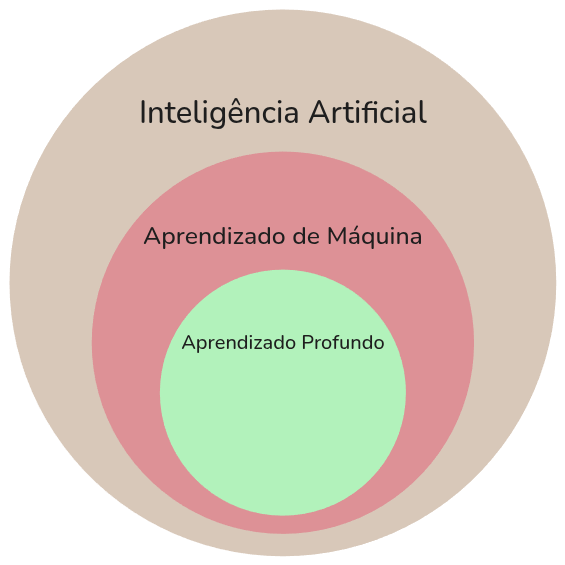
\includegraphics[width=0.4\linewidth]{venn-ai.png}
    \label{fig:hierarquia_ia}
    \legend{Fonte - Elaborado pelo autor.}
\end{figure}

Dessa forma, o DL estabelece a base teórica para o desenvolvimento de sistemas de visão computacional capazes de analisar sequências de vídeo de forma automática, sendo a base metodológica deste trabalho.

\section[Aprendizado Supervisionado e Classificação Binária]{Aprendizado Supervisionado e Classificação Binária}

O treinamento de modelos de DL para tarefas de visão computacional é, em grande parte, realizado sob o paradigma de Aprendizado Supervisionado (\textit{Supervised Learning} – SL). Nessa abordagem o modelo é treinado a partir de um conjunto de dados rotulado, no qual cada instância de entrada $ x $ está associada a um rótulo de saída conhecido $ y $, frequentemente denominado \textit{ground truth}. O objetivo do processo de aprendizado é estimar uma função de mapeamento $f \colon X \to Y$ capaz de generalizar adequadamente para dados não observados, minimizando o erro entre as predições do modelo e os rótulos reais \cite{found}.

Dentre as diversas tarefas que podem ser realizadas com SL, a classificação destaca-se como uma das mais recorrentes. Na classificação o objetivo é atribuir cada entrada a uma dentre um conjunto finito de classes discretas \cite{ibm}. No contexto deste trabalho, a tarefa abordada consiste em um problema de classificação binária, no qual o espaço de saída é composto por duas classes mutuamente exclusivas: “\textit{Shoplifting}” e “Normal”. Formalmente, a classificação binária pode ser modelada como a predição de uma variável aleatória $y \in \{0,1\}$, sendo que, por convenção, a classe positiva ($y=1$) representa o evento de interesse e a classe negativa ($y=0$) representa eventos normais. A saída do modelo é tipicamente interpretada como uma probabilidade associada à classe positiva, permitindo a definição de um limiar de decisão para a classificação final \cite{supervised}.

Um aspecto fundamental do tipo de problema abordado no presente trabalho é o desbalanceamento de classes: eventos de interesse, como furtos, ocorrem com frequência significativamente menor em comparação a comportamentos normais. Como consequência, um modelo treinado de forma ingênua pode apresentar viés em direção à classe majoritária (i.e. “Normal”), resultando em predições aparentemente precisas em termos de acurácia, mas pouco eficazes na detecção do evento raro \cite{desbal}. Desta forma, torna-se necessário adotar estratégias que mitiguem os efeitos do desbalanceamento, incluindo o uso de funções de perda apropriadas e métricas de avaliação mais informativas, capazes de refletir o desempenho do modelo em ambas as classes \cite{metrics}. Esses aspectos são fundamentais para a correta avaliação de sistemas de detecção de eventos raros e serão discutidos em maior detalhe nas seções subsequentes.

\section[Análise de Imagens]{Análise de Imagens}

No contexto do DL, imagens são representadas como tensores multidimensionais, nos quais cada elemento corresponde à intensidade de um pixel em determinado canal de cor, tipicamente no espaço RGB. A partir dessa representação estruturada, modelos computacionais são capazes de extrair padrões relevantes por meio de transformações sucessivas aplicadas aos dados de entrada \cite{vision}.

Dentre as abordagens desenvolvidas para tarefas de classificação, destacam-se duas famílias principais de modelos: as RNCs e os modelos baseados em Transformadores de visão. Essas abordagens diferem fundamentalmente na forma como capturam dependências espaciais e semânticas nas imagens, constituindo paradigmas complementares na área de visão computacional.

\subsection[Redes Neurais Convolucionais]{Redes Neurais Convolucionais}

As RNCs foram projetadas para explorar a estrutura espacial das imagens, incorporando propriedades como localidade e invariância à translação. Diferentemente de redes totalmente conectadas, nas quais cada neurônio se conecta a todos os elementos da entrada, as RNCs utilizam filtros convolucionais que operam localmente sobre regiões da imagem, reduzindo significativamente o número de parâmetros e preservando a organização espacial dos dados \cite{vision}.

A operação central dessas redes é a convolução, na qual um conjunto de filtros aprendíveis é aplicado de forma deslizante sobre a imagem, gerando mapas de características. Esses mapas capturam padrões locais, como bordas, texturas e formas, que são progressivamente combinados em representações mais abstratas ao longo das camadas mais profundas da rede. Como resultado, as RNCs aprendem uma hierarquia de características, partindo de informações de baixo nível até representações semânticas de alto nível \cite{goodfellow}.

A \autoref{fig:cnn_arquitetura} ilustra visualmente essa dinâmica, na qual a imagem de entrada é submetida a sucessivas camadas de convolução e \textit{pooling}, responsáveis por extrair os mapas de características (\textit{features}) de forma hierárquica. Ao término dessa fase de extração, essas informações espaciais são unidas e repassadas para a etapa de classificação, onde a rede consolida os dados para prever a saída final.

\begin{figure}[!ht]
    \centering
    \caption[Arquitetura típica de uma RNC e a extração progressiva de mapas de características.]{Arquitetura típica de uma RNC e a extração progressiva de mapas de características.}
    \label{fig:cnn_arquitetura}
	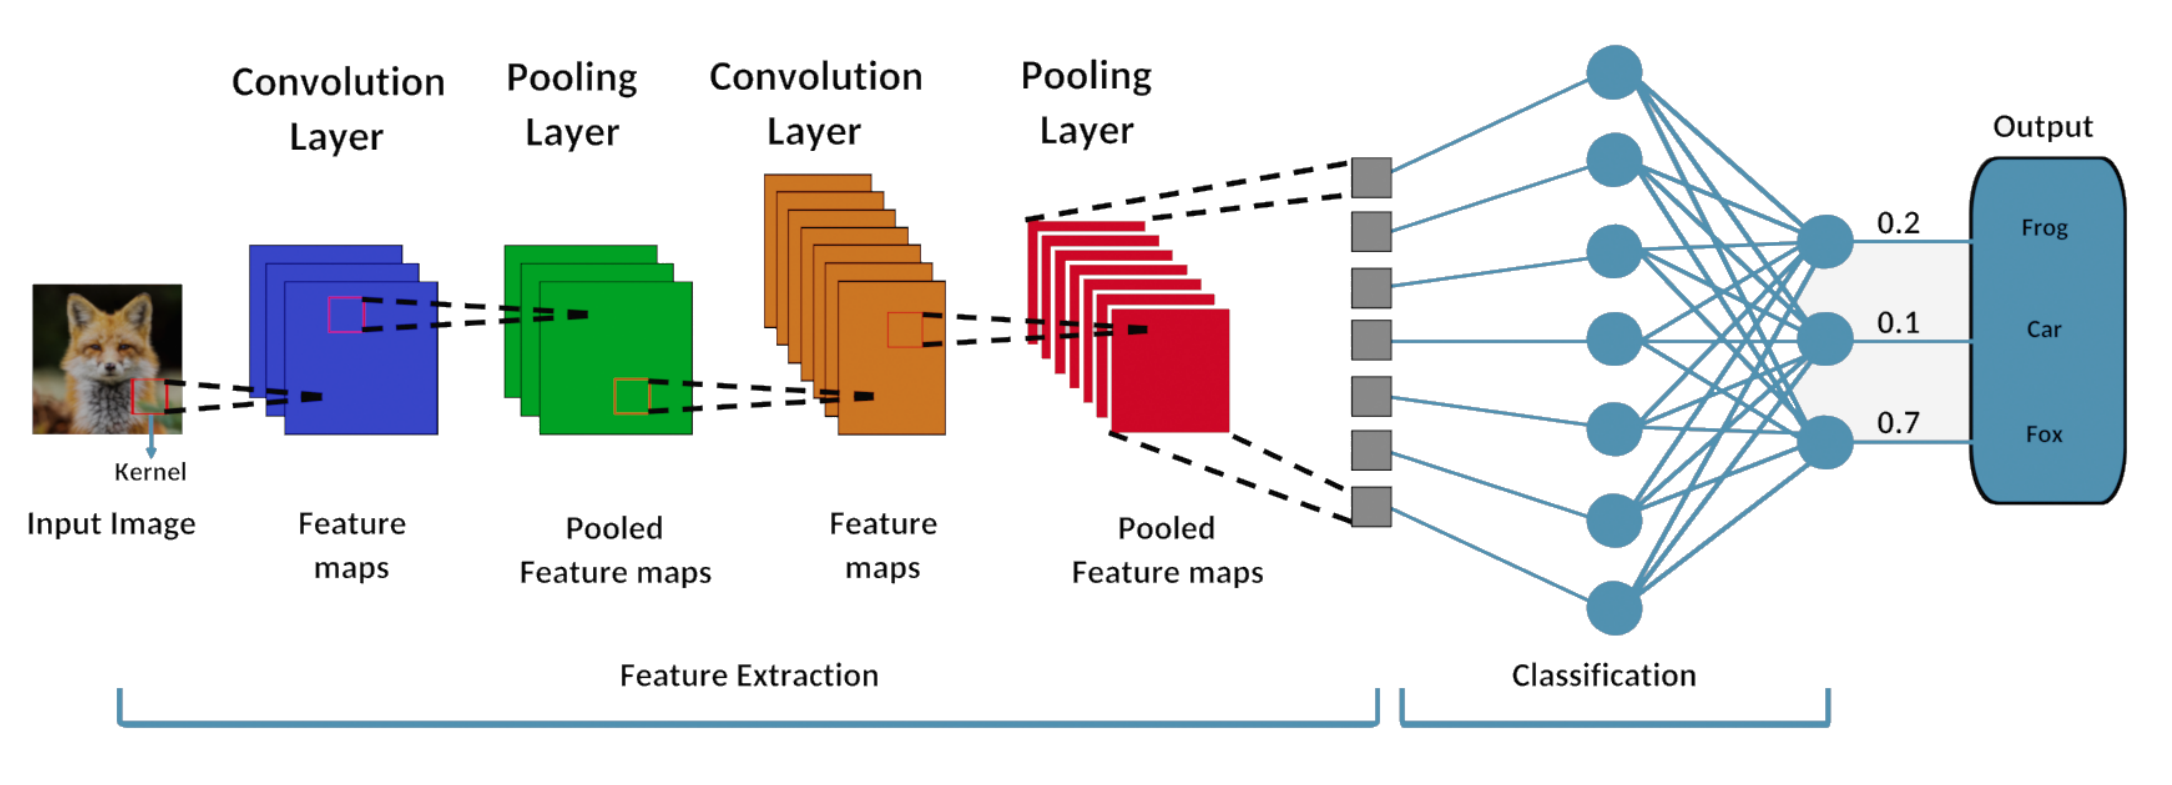
\includegraphics[width=1.0\linewidth]{cnn.png}
	\legend{Fonte - \citeonline{cnn_image}.}
\end{figure}

\subsection[Transformadores de Visão]{Transformadores de Visão}

Os transformadores de visão são baseados em mecanismos de atenção adotando uma abordagem global para a análise de imagens. Os \textit{Transformers} adaptados para tarefas de visão computacional, como o \textit{Vision Transformer} (ViT) \cite{vitmetrics}, dividem a imagem em pequenas regiões chamadas \textit{patches}, que são tratadas como elementos de uma sequência. Cada \textit{patch} é projetado em um espaço vetorial, permitindo que o modelo processe a imagem de forma análoga a uma sequência de \textit{tokens}. Para preservar a informação espacial, são adicionados \textit{embeddings} posicionais que codificam a localização original de cada fragmento na imagem \cite{attentionall}.

Na \autoref{fig:vit_img}, observa-se o fluxo de processamento. A imagem de entrada é fragmentada e alinhada em diversos \textit{patches}. Esses fragmentos são combinados com as informações de localização (\textit{Positional embedding}). O modelo então analisará as relações entre essas partes para gerar a classificação final, através de camadas de  mecanismos de atenção (\textit{Multi-head attention}) e normalizações.


\begin{figure}[!ht]
    \centering
    \caption[Processo de divisão de uma imagem em \textit{patches} e adição de \textit{embeddings} posicionais na arquitetura \textit{Vision Transformer}.]{Processo de divisão de uma imagem em \textit{patches} e adição de \textit{embeddings} posicionais na arquitetura \textit{Vision Transformer}.}
	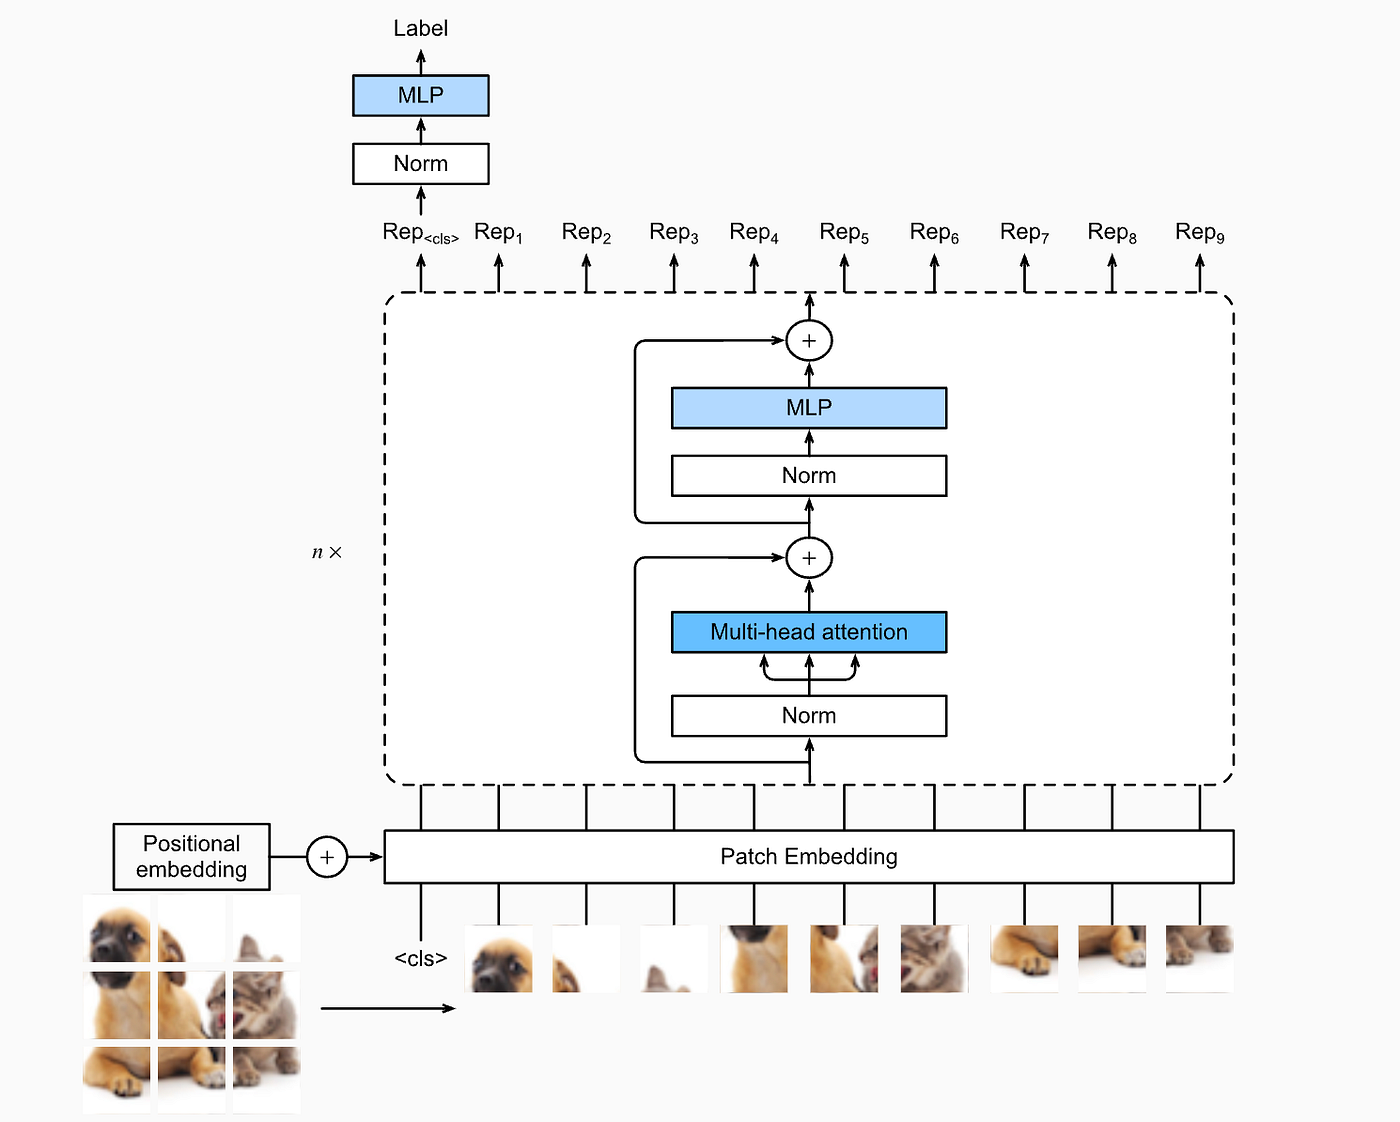
\includegraphics[height=0.7\linewidth]{vit.png}
    \label{fig:vit_img}
	\legend{Fonte - \citeonline{vit_img}.}
\end{figure}

O principal mecanismo desses modelos é a atenção (\textit{self-attention)}, que permite ao modelo calcular dinamicamente a relevância entre diferentes regiões da imagem \cite{comparing}. Dessa forma, cada parte da imagem pode interagir diretamente com todas as demais, possibilitando a captura de dependências globais desde as primeiras camadas da rede. Essa característica representa uma vantagem significativa em tarefas que exigem compreensão contextual ampla, como é o caso do monitoramento de lojas de varejo a partir de imagens de CFTV \cite{comparing2}.

\section[Análise de Vídeos]{Análise de Vídeos}

A análise de vídeos difere fundamentalmente da análise de imagens estáticas por incorporar a dimensão temporal como elemento essencial para a compreensão dos dados. Dessa forma, a representação de dados de entrada em modelos de aprendizado profundo é estendida para tensores multidimensionais que incluem a dimensão temporal. Isto é, um vídeo pode ser modelado como uma sequência ordenada de quadros, na qual cada quadro contribui para a construção de um padrão dinâmico ao longo do tempo \cite{representation}.

Para solução dessa diferença fundamental e modelagem espaço-temporal dos vídeos, duas abordagens são utilizadas majoritariamente: as RNCs 3D e os modelos de vídeo baseados em mecanismos de atenção. Assim como no 2D, as abordagens diferem principalmente na forma como capturam relações espaciais e temporais.

As RNCs 3D estendem diretamente o conceito de convolução bidimensional para o domínio espaço-temporal. Nessa abordagem, os filtros convolucionais passam a operar simultaneamente nas dimensões de altura, largura e tempo, permitindo que o modelo extraia características dinâmicas a partir de volumes de dados \cite{video_conv}. Dessa forma, padrões de movimento são aprendidos de forma integrada à informação espacial presente nos quadros. Essas redes preservam o viés indutivo das convoluções, como a localidade e a invariância à translação, agora estendidas ao domínio temporal. Isso permite que essas arquiteturas capturem de forma eficiente padrões locais de movimento ao longo de sequências curtas de quadros. No entanto, a modelagem de dependências temporais de longo alcance depende do empilhamento de múltiplas camadas, o que pode aumentar significativamente a complexidade do modelo e dificultar o treinamento. Além disso, a introdução da dimensão temporal nos filtros resulta em um crescimento expressivo no número de parâmetros, elevando o custo computacional de inferência e de treino \cite{rnc_3d}.

Os modelos de vídeo baseados em mecanismos de atenção estendem a arquitetura dos \textit{Transformers} para incorporar explicitamente a dimensão temporal na modelagem dos dados. Para vídeos, a sequência de entrada passa a incluir múltiplos quadros, exigindo a modelagem conjunta de relações espaciais e temporais \cite{timesformer}. Seria possível adaptar os modelos 2D aplicando diretamente o mecanismo de \textit{self-attention} sobre todos os \textit{patches} de todos os quadros simultaneamente. No entanto, essa estratégia apresenta custo computacional elevado, uma vez que a complexidade da atenção cresce quadraticamente com o número de elementos da sequência. Para contornar essa limitação, arquiteturas modernas propõem a fatoração da atenção em componentes espaciais e temporais, permitindo modelar essas dimensões de forma separada e mais eficiente. Nesse contexto, a atenção temporal permite capturar relações entre diferentes instantes do vídeo, identificando padrões dinâmicos ao longo do tempo, enquanto a atenção espacial foca na interação entre regiões dentro de um mesmo quadro \cite{vivit}. 

\section[Arquiteturas para Análise de Vídeos]{Arquiteturas para Análise de Vídeos}

 O uso de arquiteturas consolidadas na literatura e amplamente adotadas em aplicações práticas permite o aproveitamento de pesos pré-treinados em grandes bases de dados, reduzindo o custo computacional e a necessidade de grandes volumes de dados rotulados. Esse aspecto é particularmente relevante em cenários aplicados, nos quais a disponibilidade de dados específicos pode ser limitada. Nesse contexto, este trabalho adota duas arquiteturas já consolidadas para a análise de vídeos: o I3D (\textit{Inflated 3D ConvNet}) e o TimeSFormer. A escolha dessas arquiteturas permite a comparação entre abordagens com diferentes vieses indutivos e capacidades de modelagem, conforme discutido nas seções anteriores.

\subsection[\textit{Inflated 3D ConvNet}]{\textit{Inflated 3D ConvNet}}

O modelo I3D estende arquiteturas convolucionais 2D para o domínio espaço-temporal por meio da chamada inflação de filtros. Nesse processo, filtros bidimensionais previamente treinados em tarefas de classificação de imagens são expandidos para três dimensões, permitindo sua aplicação direta sobre sequências de vídeo. A \autoref{fig:comp_conv_2d_3d} apresenta a convolução 2D, que atua apenas sobre as dimensões espaciais de altura e largura, e a convolução 3D, que incorpora a dimensão de profundidade, ou seja, o tempo no contexto dos vídeos, possibilitando a extração simultânea de características espaciais e temporais.

\begin{figure}[!ht]
    \centering
    \caption[Comparação entre a operação de convolução padrão (2D) e a convolução espaço-temporal (3D) aplicada a volumes de vídeo.]{Comparação entre a operação de convolução padrão (2D) e a convolução espaço-temporal (3D) aplicada a volumes de vídeo.}
	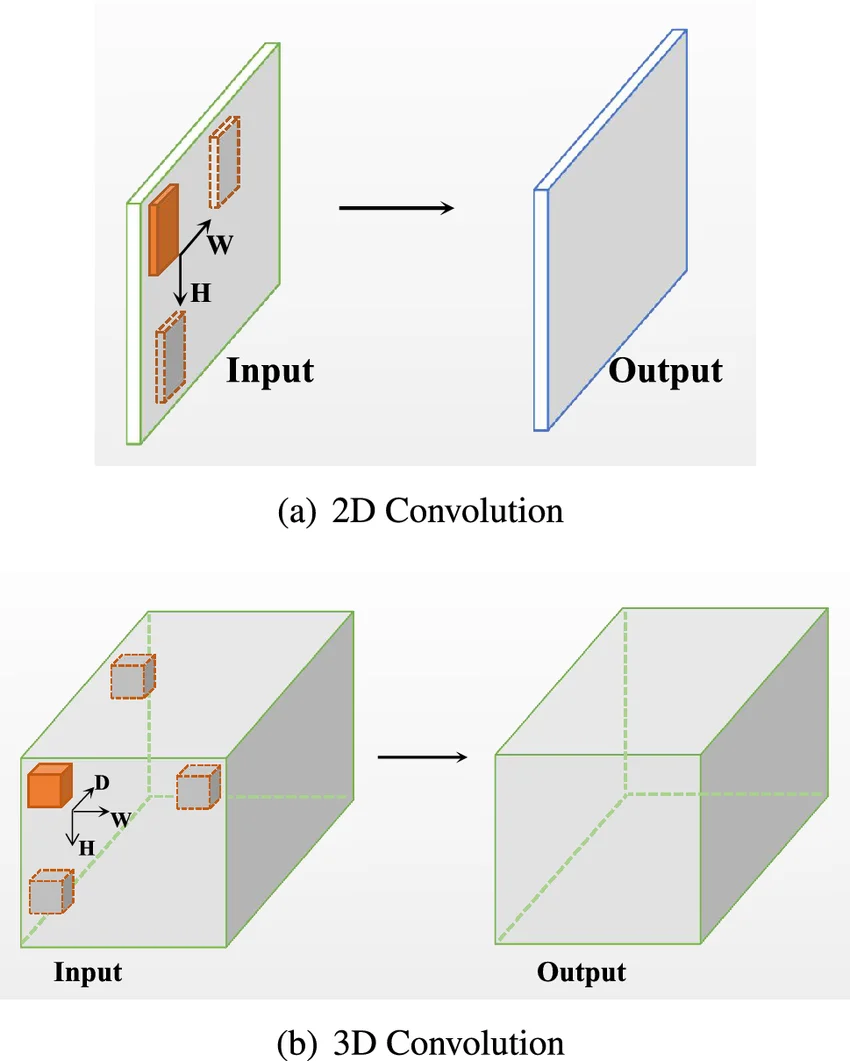
\includegraphics[height=0.65\linewidth]{figuras/3d-vs-2d.png}
    \label{fig:comp_conv_2d_3d}
	\legend{Fonte - \citeonline{3dcnn_img}.}
\end{figure}

Uma vantagem importante do I3D é a possibilidade de inicialização a partir de pesos pré-treinados em grandes bases de imagens, o que facilita o treinamento e melhora a capacidade de generalização. Além disso, sua estrutura baseada em convoluções 3D permite capturar eficientemente padrões locais espaço-temporais \cite{i3d}.

Por outro lado, assim como outras arquiteturas baseadas em convoluções tridimensionais, o I3D apresenta limitações na modelagem de dependências de longo alcance, além de um custo computacional elevado decorrente do aumento do número de parâmetros.

\subsection[TimeSFormer]{TimeSFormer}

O TimeSFormer adapta a arquitetura dos \textit{Transformers} para a análise de vídeos, explorando mecanismos de \textit{self-attention} para modelar relações espaço-temporais, sendo capaz de estabelecer interações diretas entre diferentes regiões e instantes do vídeo. 

Assim como outros modelos baseados em \textit{Transformers}, o TimeSFormer representa os dados de entrada como sequências de \textit{patches} extraídos dos quadros do vídeo, incorporando informações posicionais para preservar a estrutura espaço-temporal. No entanto, diferentemente dos modelos comuns do mesmo tipo, aqui a atenção é aplicada em diferentes graus ao longo do tempo e do espaço, isto é: ao invés de utilizar todos os \textit{patches} no quadro atual, anterior e posterior para classificação do quadro atual como na \textit{Joint Space-Time Attention} da \autoref{fig:timesformer_attention}, o TimeSFormer utiliza um subconjunto deste, como na abordagem \textit{Divided Space-Time Attention}, permitindo reduzir o custo computacional sem detrimento significativo da performance \cite{timesformer}.

\begin{figure}[!ht]
    \centering
    \caption[Visualização da fatoração do mecanismo de atenção em componentes temporais e espaciais na arquitetura TimeSFormer.]{Visualização da fatoração do mecanismo de atenção em componentes temporais e espaciais na arquitetura TimeSFormer.}
	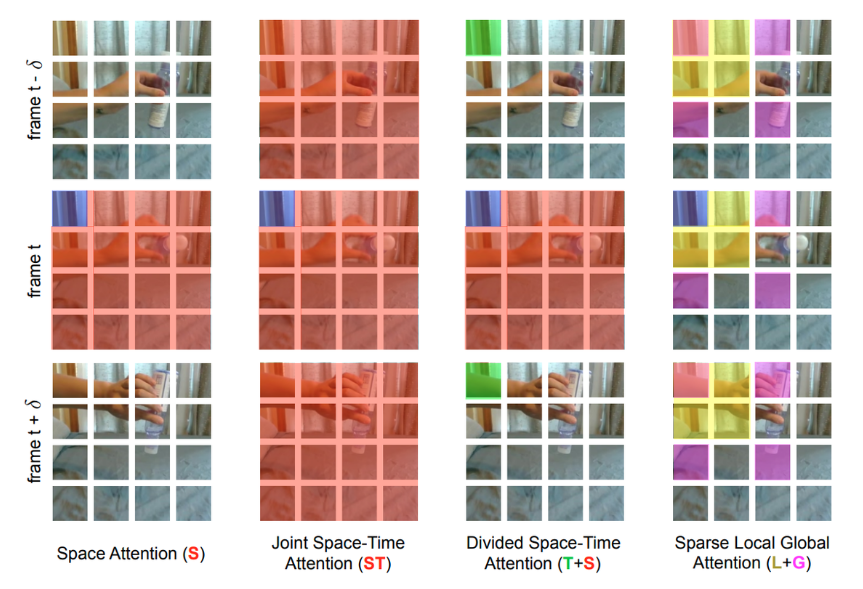
\includegraphics[height=0.54\linewidth]{figuras/timesformer.png}
    \label{fig:timesformer_attention}
	\legend{Fonte - Adaptado de \citeonline{timesformer}.}
\end{figure}

\section[\textit{Transfer Learning} e \textit{fine-tuning}]{\textit{Transfer Learning} e \textit{fine-tuning}}

O treinamento de modelos de aprendizado profundo para tarefas de visão computacional, especialmente no domínio de vídeos, demanda grandes volumes de dados rotulados e elevado custo computacional. Para mitigar esse problema, técnicas de \textit{Transfer Learning} surgem como uma abordagem eficaz, consistindo na reutilização do conhecimento adquirido em grandes domínios de origem para acelerar a convergência e melhorar a generalização em novas tarefas \cite{pan2010survey}. Nestas técnicas assume-se que representações genéricas, como bordas em imagens ou noções básicas de movimento, são transferíveis para problemas específicos, o que é vital quando os conjuntos de dados alvo são limitados \cite{yosinski2014how}.

Tanto o I3D quanto o TimeSFormer, adotados neste trabalho, possuem versões com pesos pré-treinados em grandes conjuntos de dados de vídeo, o que permite sua adaptação para tarefas específicas com menor quantidade de dados. Para o I3D, os pesos inicias surgem à partir da inflação de filtros 2D originalmente treinados no conjunto de dados ImageNet para a dimensão 3D, seguidos de um pré-treinamento no banco de dados Kinetics-400 (K400). O K400 é um banco de dados abrangente composto por centenas de milhares de vídeos focados em ações humanas. Essa abordagem em duas etapas garante que o I3D pré-treinado herde a forte capacidade de extração de características espaciais do ImageNet e, simultaneamente, aprenda a modelar dinâmicas temporais no domínio de vídeos \cite{deng2009imagenet, kay2017kinetics}.

Já o TimeSFormer possui pesos pré-treinados no K400 e no Something-Something V2 (SSv2). A escolha de disponibilizar pesos para esses dois bancos de dados baseia-se nas diferenças cruciais entre eles.
O K400 possui um forte viés espacial, onde a presença de objetos e o cenário muitas vezes bastam para inferir a ação. Em contraste, o SSv2 foca em interações abstratas e direcionais, onde a compreensão da ordem e evolução temporal é obrigatória para o reconhecimento correto \cite{kay2017kinetics, goyal2017something}.

A disponibilidade desses pesos pré-treinados é particularmente relevante em cenários aplicados, nos quais os conjuntos de dados específicos são significativamente menores. No entanto, nessas situações o uso direto dos modelos pré-treinados não é suficiente, uma vez que as distribuições de dados e os padrões de interesse diferem daqueles presentes nos conjuntos de origem. Dessa forma, torna-se necessário adaptar os modelos ao novo domínio por meio do processo de \textit{fine-tuning}, que  consiste no ajuste dos parâmetros de um modelo previamente treinado utilizando um novo conjunto de dados, com o objetivo de especializar as representações aprendidas para a tarefa alvo. Diferentemente do treinamento do zero, essa abordagem parte de um estado inicial já informativo, permitindo uma convergência mais rápida e, frequentemente, melhor desempenho final \cite{tajbakhsh2016convolutional}.

Esse processo pode ser realizado de diferentes maneiras, dependendo do grau de adaptação desejado. Em uma abordagem mais conservadora, as camadas iniciais do modelo são mantidas congeladas, enquanto apenas as camadas finais são treinadas. Alternativamente, é possível realizar o ajuste completo de todos os parâmetros da rede, permitindo uma adaptação mais profunda ao novo domínio, ao custo de maior risco de \textit{overfitting} \cite{yosinski2014how}.

A \autoref{fig:finetune} sintetiza visualmente a união desses conceitos. Como demonstrado, o modelo adquire conhecimento inicial a partir de um grande volume de dados, estabelecendo pesos pré-treinados em suas camadas em comum. Ao ser transferido para uma nova tarefa com dados mais escassos, as camadas que diferem das originais passam pelo \textit{fine-tuning}, permitindo adaptar as representações do modelo para gerar a saída específica sem treinamento do início.

\begin{figure}[!ht]
    \centering
    \caption[Fluxo conceitual do processo de \textit{Transfer Learning} e \textit{fine-tuning} adaptando pesos de um domínio de origem para uma tarefa específica.]{Fluxo conceitual do processo de \textit{Transfer Learning} e \textit{fine-tuning} adaptando pesos de um domínio de origem para uma tarefa específica.}
	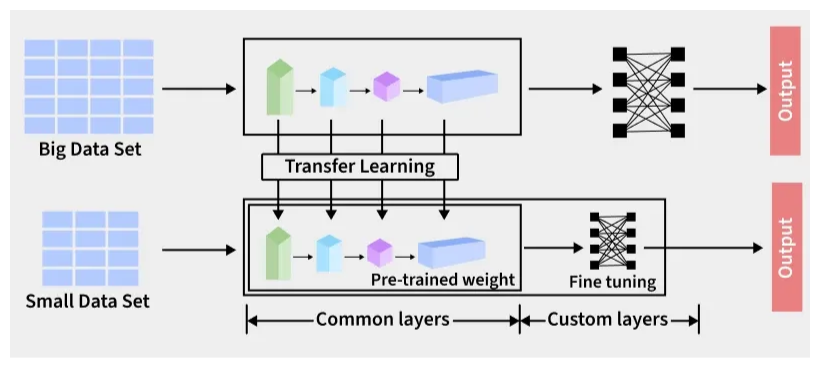
\includegraphics[height=0.35\linewidth]{figuras/transfer-fine.png}
    \label{fig:finetune}
	\legend{Fonte - \citeonline{gfg_finetuning}.}
\end{figure}

\section[Métricas e Função de Perda]{Métricas e Função de Perda}

O treinamento de modelos de aprendizado profundo para classificação de vídeos requer a definição simultânea de dois componentes fundamentais: a função de perda, responsável por guiar o processo de otimização dos parâmetros da rede, e as métricas de avaliação, utilizadas para quantificar o desempenho do modelo de forma interpretável e comparável \cite{metrics}. Em uma classificação binária sob forte desbalanceamento de classes tanto a escolha da função de perda quanto das métricas de avaliação é de extrema importância a fim de evitar vieses em direção à classe majoritária.

A função de perda atua como um mecanismo de retroalimentação do modelo, mensurando o erro entre as predições realizadas e os rótulos reais, permitindo a atualização dos pesos por meio do algoritmo de retropropagação \cite{goodfellow}.

Para o modelo I3D, cuja saída consiste em uma única probabilidade associada à ocorrência da classe positiva, é empregada uma função de perda apropriada para problemas binários, a \textit{Binary Cross-Entropy} (BCE), baseada na comparação direta entre a probabilidade predita e o rótulo verdadeiro. Essa escolha é coerente com a modelagem probabilística do problema e favorece a penalização mais intensa de predições incorretas realizadas com alta confiança. Por sua vez, no modelo TimeSFormer, cuja saída é estruturada como um vetor de probabilidades para duas classes, utiliza-se uma função de perda de natureza categórica, a \textit{Cross-Entropy Loss} (CEL), que considera simultaneamente as probabilidades atribuídas a cada classe possível. Embora as formulações matemáticas dessas funções difiram, ambas compartilham o mesmo objetivo fundamental: maximizar a probabilidade da classe correta enquanto minimizam a da classe incorreta \cite{ibm}.

Considerando o desbalanceamento inerente ao problema, são adotadas estratégias de ponderação das classes durante o cálculo da perda, nas quais a penalização atribuída aos erros é proporcional ao grau de sub-representação da classe, sendo mais severa quanto mais minoritária ela for. Essa abordagem é essencial para evitar que o modelo aprenda soluções triviais, como a predição constante da classe majoritária, o que resultaria em desempenho aparente elevado, porém sem utilidade prática \cite{desbal}.

No que diz respeito à avaliação de desempenho, métricas derivadas da matriz de confusão, como precisão e revocação, permitem analisar diferentes aspectos do comportamento do modelo, como sua capacidade de evitar falsos positivos ou de identificar corretamente eventos de interesse. A partir dessas duas medidas, calcula-se o F1-Score, que consiste na média harmônica entre a precisão e a revocação, sendo assim uma métrica amplamente utilizada para resumir o equilíbrio do classificador em um único valor. No entanto, em cenários desbalanceados, a acurácia, revocação ou F1-Score isoladamente podem ser medidas enganosas, não refletindo adequadamente o desempenho sobre a classe minoritária.

Por este motivo, adota-se como principal métrica de avaliação a área sob a curva ROC (\textit{Area Under the Receiver Operating Characteristic Curve} - AUC-ROC). A curva ROC ilustra o desempenho do classificador ao plotar a taxa de verdadeiros positivos contra a taxa de falsos positivos ao longo de diferentes limiares de decisão. A AUC-ROC resume essa curva em um único valor, que quantifica a capacidade do modelo de discriminar entre as classes variando de 0 a 1. Deste modo, quanto mais próximo de 1 o AUC-ROC, melhor o desempenho do modelo, sendo 1 correspondente a um classificador perfeito, enquanto um valor de 0,5 indica uma classificação aleatória, como mostra a \autoref{fig:roc}. O uso dessa métrica mostra-se especialmente adequado por sua independência de um limiar fixo e por capturar com clareza a relação de compromisso entre acertos e falsos alarmes \cite{metrics}.

Adicionalmente, após o treinamento, os melhores modelos são avaliados em um mesmo conjunto de teste, previamente separado do processo de otimização, permitindo uma comparação justa entre diferentes arquiteturas e estratégias de treinamento. Essa abordagem assegura que a escolha da melhor configuração não esteja enviesada por dados utilizados durante o ajuste dos parâmetros, promovendo maior confiabilidade na análise dos resultados. Nesta etapa, devido ao fato de falsos negativos serem mais críticos para o cenário de detecção de furtos, o F2-Score, que atribui mais peso à revocação, é preferível como métrica de avaliação final.

\begin{figure}[!ht]
    \centering
    \caption[Exemplo de Curvas ROC, a Área Sob a Curva (AUC) é a métrica empregada para avaliar cenários de classificação desbalanceados.]{Exemplo de Curvas ROC, a Área Sob a Curva (AUC) é a métrica empregada para avaliar cenários de classificação desbalanceados.}
	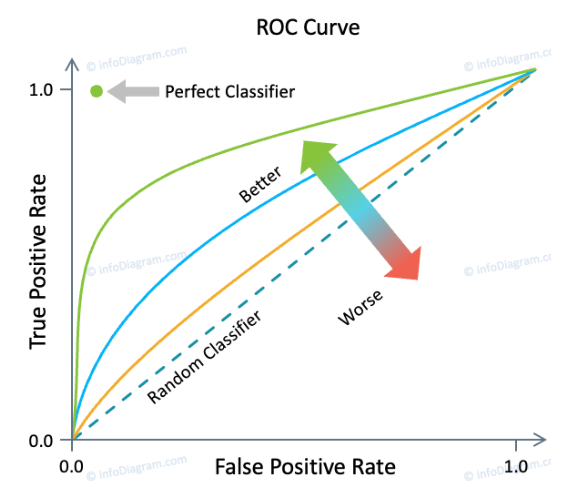
\includegraphics[height=0.5\linewidth]{figuras/roc.png}
	\legend{Fonte - Adaptado de \citeonline{infodiagram_auc_roc}.}
    \label{fig:roc}
\end{figure}

Por fim, aspectos relacionados à estabilidade do treinamento também desempenham papel relevante no desempenho final dos modelos. O I3D incorpora mecanismos de normalização baseados em estatísticas do \textit{batch}, em contrapartida com o TimeSFormer, que utiliza estratégias alternativas de normalização, mais adequadas à sua estrutura baseada em mecanismos de atenção \cite{i3d,timesformer}. Essas diferenças estruturais impactam diretamente a dinâmica de treinamento e devem ser consideradas na definição dos hiperparâmetros como a taxa de aprendizado inicial.
%TCC:

\chapter[Descrição do Banco de Dados]{Descrição do Banco de Dados}

O desempenho de modelos de aprendizado profundo em tarefas de classificação de vídeos está diretamente relacionado à qualidade, diversidade e representatividade do conjunto de dados utilizado no treinamento. No contexto da detecção de possíveis furtos no varejo, a disponibilidade de bases de dados públicas é limitada, especialmente quando se busca um equilíbrio entre realismo, anotação adequada e volume de dados. Dessa forma, optou-se pela construção de um banco de dados próprio a partir da agregação e adaptação de múltiplas fontes disponíveis na literatura.

\section[Construção do conjunto de dados]{Construção do conjunto de dados}

O conjunto de dados utilizado neste trabalho foi construído a partir da combinação de três bases públicas: DCSASS, Shoplifting Dataset 2.0 e Shoplifting Dataset MNNIT \cite{dcsass, shoplifting_20, shoplifting_mnnit}. Esses conjuntos apresentam características distintas, incluindo variações no ambiente, no tipo de anotação, na natureza dos eventos registrados e, para os casos de comportamento ilícito, nas estratégias de ocultação dos itens furtados.

Inicialmente, foram considerados os vídeos originais de cada fonte. O conjunto MNNIT é composto por 182 vídeos, sendo 90 classificados como “Normal” (i.e. ação normal de compra) e 92 como “\textit{Shoplifting}” (i.e. vídeo associado a um furto). Trata-se de um banco de dados sintético, construído com a participação de múltiplos atores em um ambiente controlado de laboratório, no qual produtos são dispostos de forma a simular um cenário de varejo. Para a classe \textit{Shoplifting}, observa-se que o padrão predominante de ocultação consiste em transportar os itens para mochilas, como na \autoref{fig:mnnit}, havendo, contudo, variação consistente quanto às características dos objetos, tais como tamanho, forma, cor, tipo e quantidade. Por outro lado, a classe “Normal” contempla interações típicas de consumidores, como observação, manuseio, retirada e devolução de um ou múltiplos itens, sendo estes iguais aos utilizados nos casos de furto. Ressalta-se ainda que as mochilas, utilizada no contexto de “\textit{Shoplifting}” como meio do ocultação, encontram-se presentes em algumas amostras da classe “Normal”, como forma de reforço positivo à semântica da ocultação, e não ao meio.

\begin{figure}[!ht]
    \centering
    \caption[Exemplo de amostra da classe “\textit{Shoplifting}” do banco de dados MNNIT.]{Exemplo de amostra da classe “\textit{Shoplifting}” do banco de dados MNNIT.}
	\includegraphics[width=\linewidth]{figuras/mnnit.png}
	\legend{Fonte - Do autor.}
    \label{fig:mnnit}
\end{figure}


O Shoplifting Dataset 2.0 tem 276 vídeos, distribuídos entre 85 “Normal”, 82 da classe “\textit{See and Let}” (Pegar e Deixar) e 109 “\textit{Shoplifting}”. A classe “\textit{See and Let}”, que representa situações em que o indivíduo manipula o produto, mas o devolve ao local de origem, foi incorporada à classe “Normal”, por não representar comportamento ilícito. Adicionalmente, a classe “\textit{Buy}” (com 66 vídeos), presente neste banco de dados, foi descartada. Tal decisão fundamenta-se no fato de que o conjunto em questão é sintético, sendo composto por encenações realizadas em um ambiente doméstico adaptado para simular o varejo, como na \autoref{fig:dataset20}. Nesse contexto, não há a representação explícita de elementos essenciais ao processo de compra real, como um ponto de pagamento. Dessa forma, as ações rotuladas como “\textit{Buy}” tornam-se semanticamente ambíguas e potencialmente indistinguíveis de comportamentos de furto, comprometendo a consistência das anotações e a confiabilidade do treinamento supervisionado.

\begin{figure}[!htbp]
    \centering
    \caption[Exemplo de amostra da classe “\textit{Shoplifting}” do banco de dados Shoplifting Dataset 2.0.]{Exemplo de amostra da classe “\textit{Shoplifting}” do banco de dados Shoplifting Dataset 2.0.}
	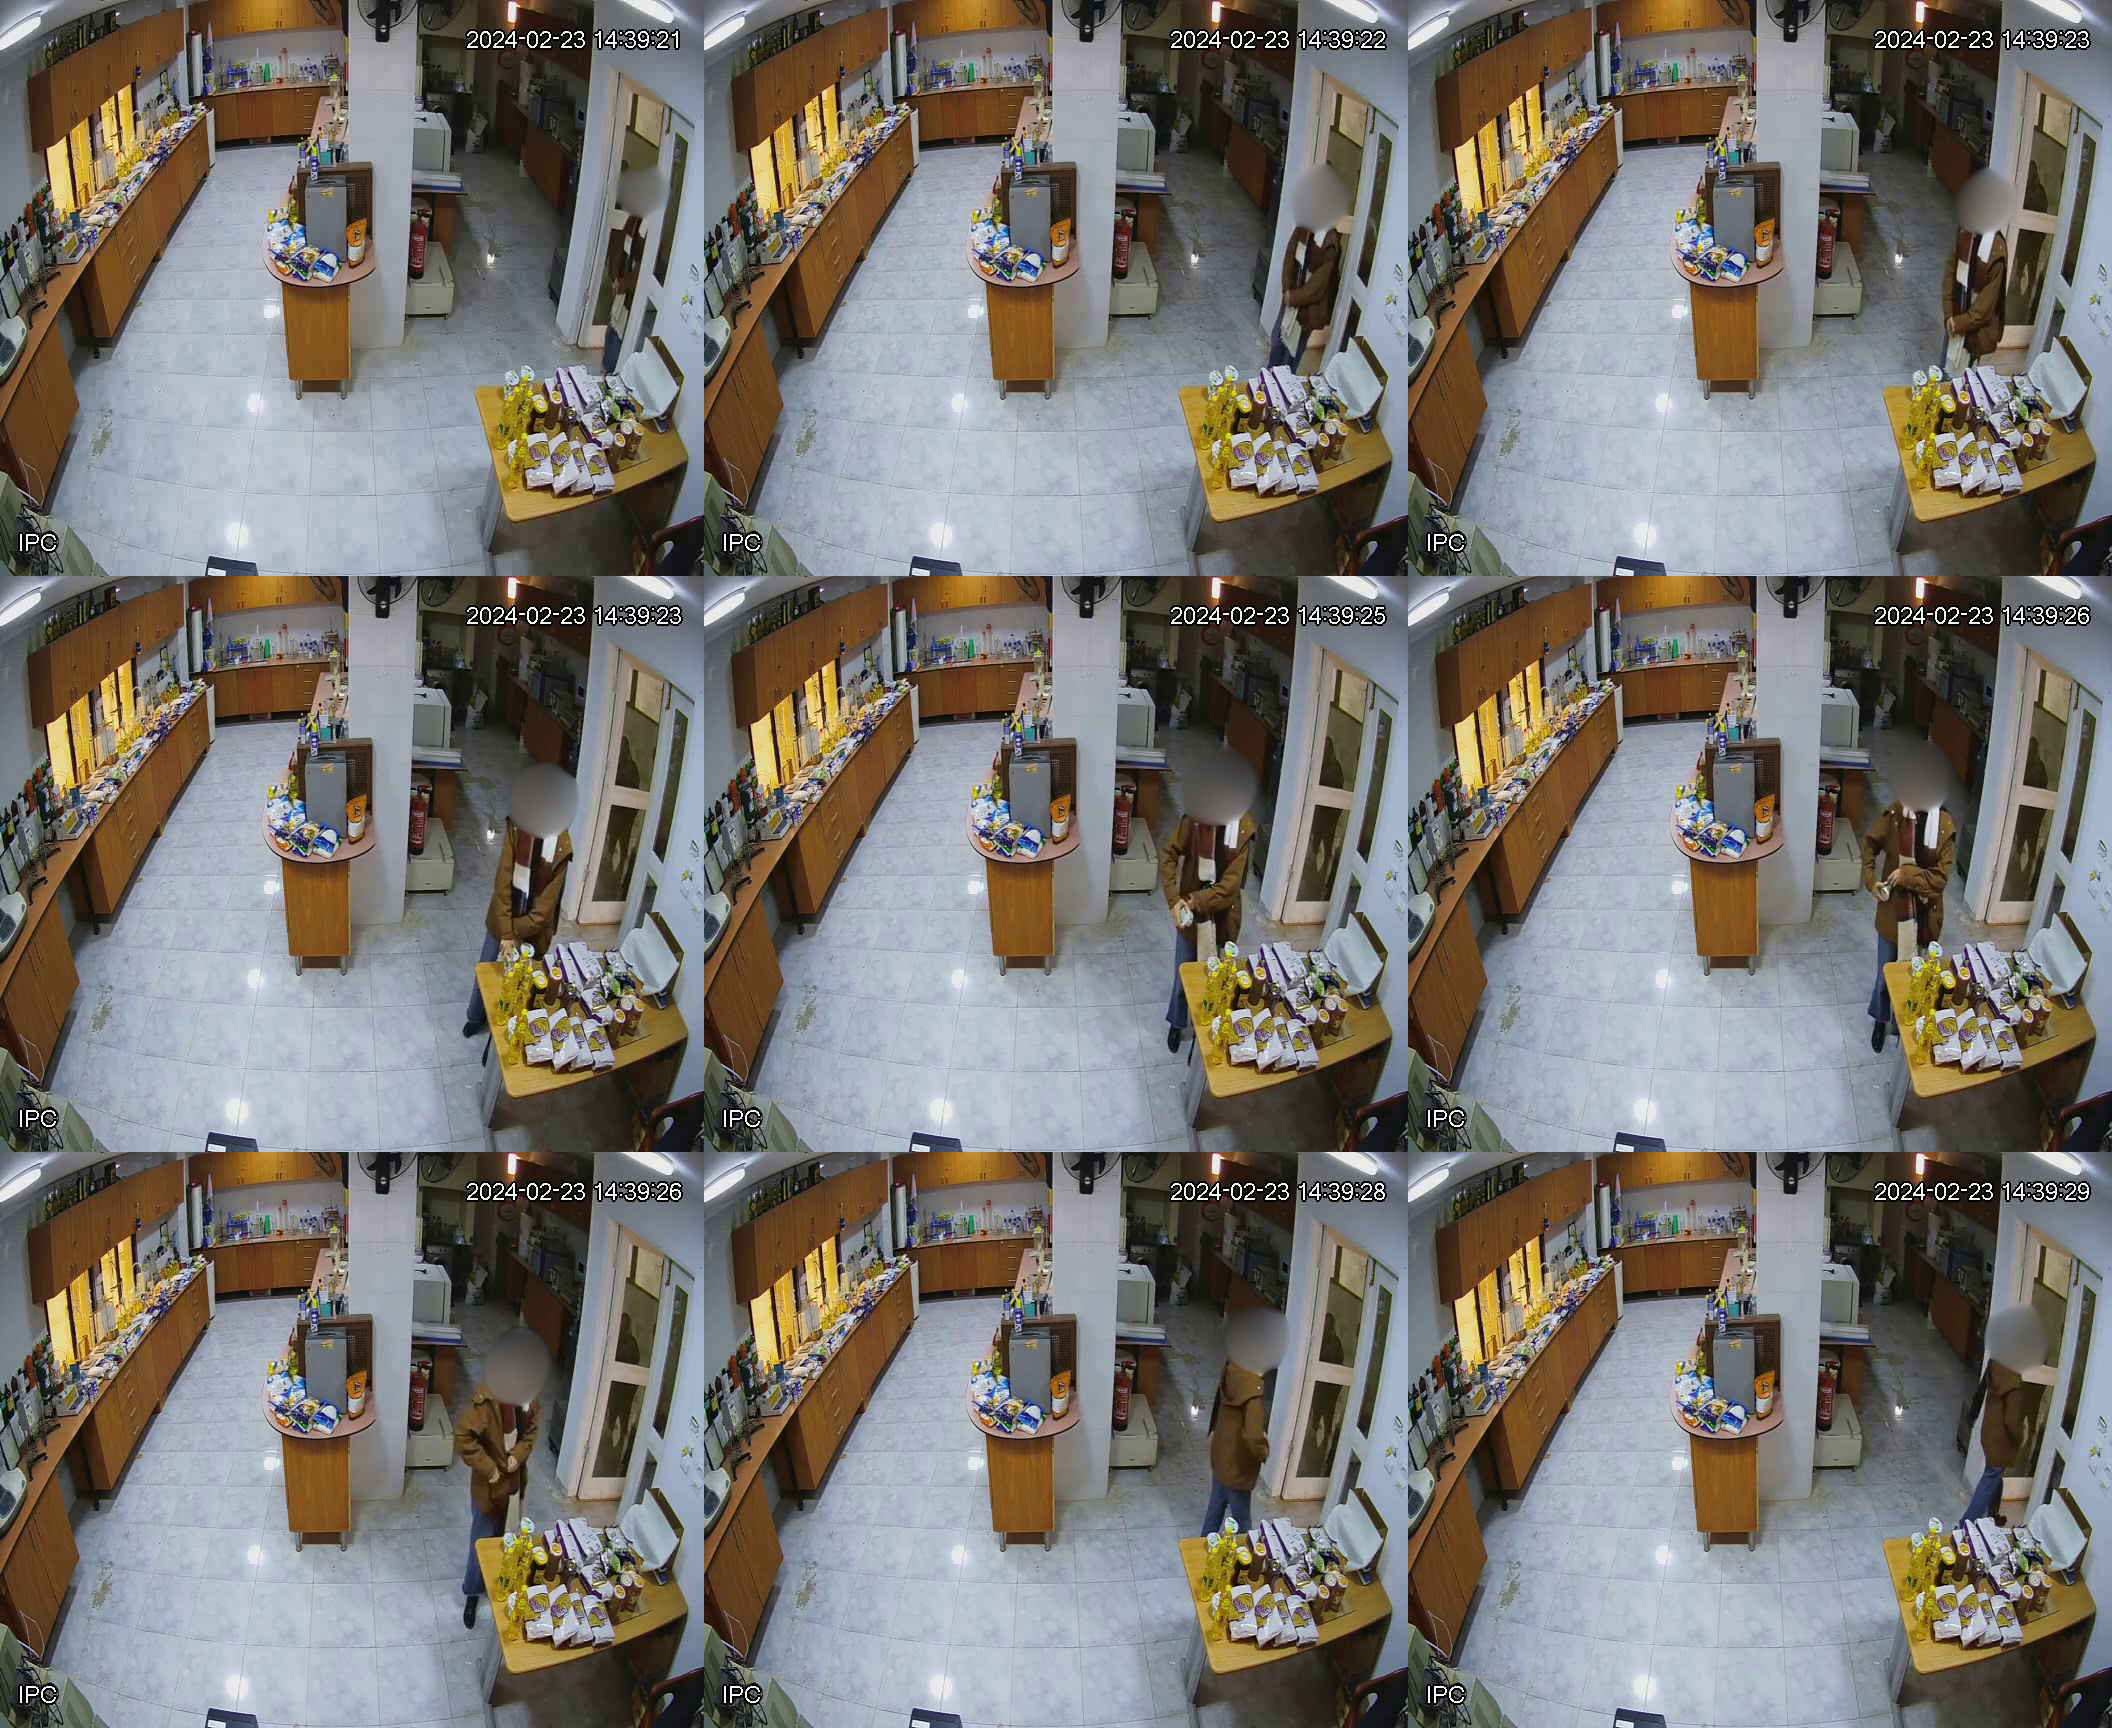
\includegraphics[width=\linewidth]{figuras/shop20.png}
	\legend{Fonte - Do autor.}
    \label{fig:dataset20}
\end{figure}

O banco de dados DCSASS, por sua vez, apresenta 28 vídeos longos contendo múltiplos eventos. Diferentemente dos demais, nesses vídeos o comportamento de furto não ocorre durante toda a duração, exigindo um processamento adicional. Assim, cada vídeo foi segmentado em múltiplos trechos menores, chamados aqui de blocos, com base nas anotações temporais disponíveis, gerando novos exemplos rotulados como “Normal” ou “\textit{Shoplifting}” conforme o rótulo dos trechos que constituem o bloco. Este processo é necessário pois, diferentemente dos anteriores, todas as amostras desse banco de dados são de ambientes e ocorrências reais, para ambas as classes. Desta forma, este conjunto é o que mais colaborou com variabilidade de ângulo de visão, ambiente, método de ocultação, item de interesse, como demonstra a \autoref{fig:dcsass} com quadros dos diferentes casos. Adicionalmente, foi realizada uma etapa de curadoria dos dados, na qual foram removidos vídeos com baixa variabilidade temporal, isto é, sequências com pouca ou nenhuma mudança significativa entre os quadros, uma vez que tais amostras não contribuem para o aprendizado de padrões dinâmicos. Como resultado, do DCSASS, foram obtidos 57 vídeos da classe “Normal” e 34 da classe “\textit{Shoplifting}”.

\begin{figure}[!htbp]
    \centering
    \caption[Exemplos de ambientes do banco de dados DCSASS.]{Exemplos de ambientes do banco de dados DCSASS.}
	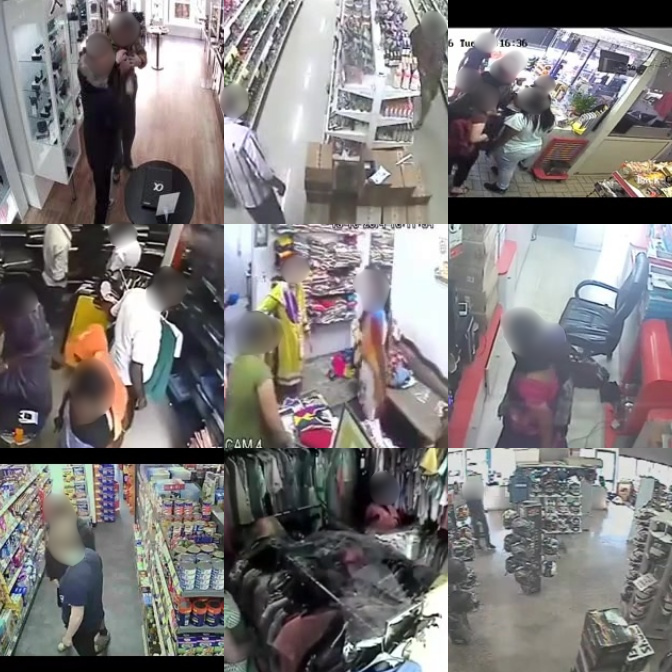
\includegraphics[width=\linewidth]{figuras/dcsass.png}
	\legend{Fonte - Do autor.}
    \label{fig:dcsass}
\end{figure}

Após o processo de agregação, filtragem e segmentação, o banco de dados final para o desenvolvimento do presente trabalho é composto por 549 vídeos, sendo 314 pertencentes à classe “Normal” e 235 à classe “\textit{Shoplifting}”. Em termos de duração, o banco totaliza aproximadamente 8031 segundos de vídeo, dos quais 5047 segundos correspondem a comportamentos normais e 2984 segundos a eventos de furto.

\section[Representação e Pré-processamento]{Representação e Pré-processamento}

Os modelos utilizados neste trabalho operam sobre sequências de quadros extraídos de vídeos, exigindo padronização das entradas em termos de resolução espacial e taxa de quadros por segundo (FPS -- \textit{Frames Per Second}) por amostra. Para cada vídeo, foi realizado um processo de reamostragem temporal, no qual o FPS original é ajustado para atender aos requisitos específicos de cada arquitetura. Em seguida, são extraídos segmentos compostos por um número fixo de quadros, correspondente ao tamanho de entrada esperado por para cada modelo em seus respectivos testes.

Cada amostra, i.e. uma sequência de quadros reamostrados de um vídeo, é tratada de forma independente sendo atribuída a um único rótulo (“Normal” ou “\textit{Shoplifting}”). Durante a fase de treinamento, os quadros são selecionados de forma variável dentro de intervalos uniformemente distribuídos ao longo do vídeo, aumentando a diversidade das amostras. Já nas etapas de validação e teste, a amostragem é realizada de forma determinística e uniforme, garantindo reprodutibilidade na avaliação. Além disso, são aplicadas transformações padrão de pré-processamento, incluindo redimensionamento espacial e normalização, de acordo com os requisitos das arquiteturas utilizadas.

\section[Aumento de Banco de Dados]{Aumento de Banco de Dados}

Com o objetivo de aumentar a capacidade de generalização dos modelos e mitigar os efeitos do tamanho limitado do conjunto de dados, foram empregadas técnicas de aumento de banco de dados durante o treinamento. Essa abordagem consiste em criar sinteticamente novas amostras para o modelo ao aplicar deformações e transformações nas imagens do conjunto de treinamento original, ensinando a rede a ser invariante a essas modificações visuais \cite{goodfellow}.

As transformações aplicadas foram variações de cor, que alteram parâmetros como brilho, contraste, saturação e matiz, e espelhamento horizontal, que introduz invariância espacial em relação à orientação da cena, com os seguintes parâmetros:

\begin{itemize}
    \item \textbf{Variação aleatória de cor (\textit{Color Jitter}):} Foram adotadas escalas de variação máxima de ± 20\% para o brilho, contraste e saturação e ± 10\% para o matiz. Essas alterações foram aplicadas de forma homogênea e simultânea a todos os quadros de uma mesma amostra temporal, mantendo a consistência temporal e evitando o efeito indesejado de cintilação.
    \item \textbf{Espelhamento horizontal (\textit{Horizontal Flip}):} Configurada com uma probabilidade de ocorrência de 50\% para cada amostra processada durante o treinamento.
\end{itemize}

A \autoref{fig:dataaug} demonstra uma sequência de quadros de um mesmo vídeo antes e depois da aplicação das transformações. Tais transformações foram selecionadas com base em sua plausibilidade no contexto real de aquisição dos dados, refletindo variações efetivamente observáveis em sistemas de câmeras, ao mesmo tempo em que evitam alterações não realistas, como o espelhamento vertical. Essas técnicas foram aplicadas de forma consistente em ambos os modelos avaliados, possuindo os mesmos parâmetros.

\begin{figure}[!htbp]
    \centering
    \caption[Exemplo de transformação de sequência de quadros original (acima) após a aplicação das técnicas adotadas para aumento de banco de dados (abaixo).]{Exemplo de transformação de sequência de quadros original (acima) após a aplicação das técnicas adotadas para aumento de banco de dados (abaixo).}
	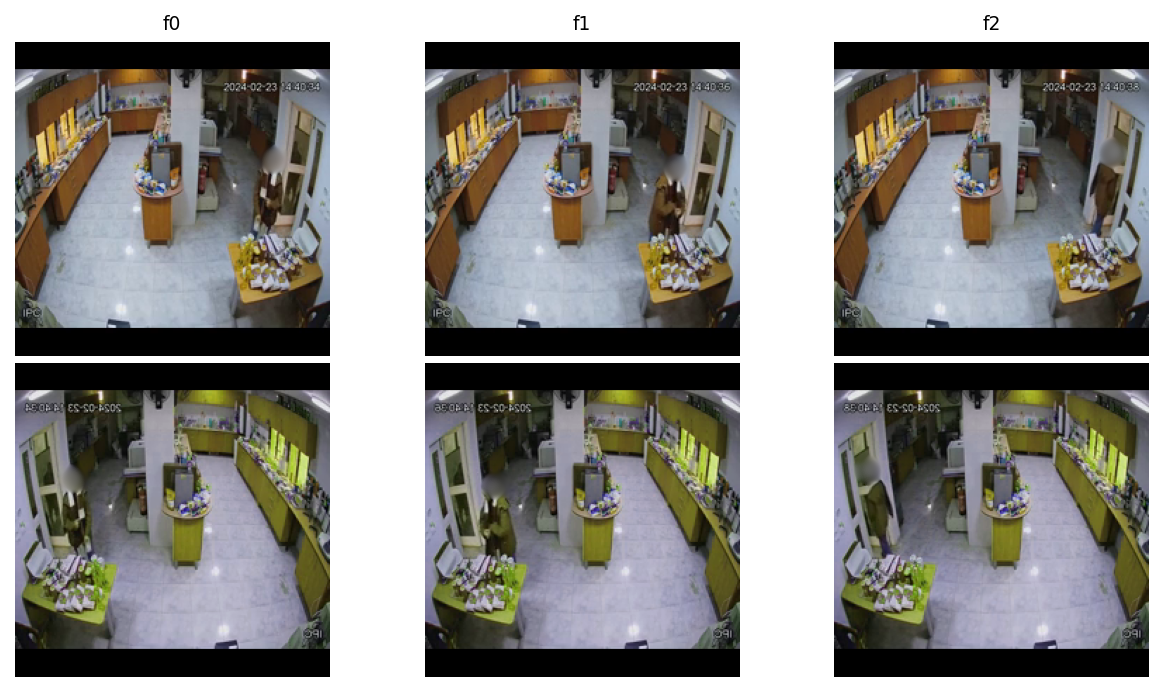
\includegraphics[width=\textwidth]{figuras/dataaug.png}
	\legend{Fonte - Do autor.}
    \label{fig:dataaug}
\end{figure}

É importante salientar que o aumento de banco de dados foi utilizado exclusivamente durante a fase de treinamento, não sendo aplicado nos conjuntos de validação e teste, a fim de preservar a integridade da avaliação e permitir uma comparação justa entre diferentes configurações.

\section[Divisão do conjunto de dados]{Divisão do Conjunto de Dados}

Como de praxe no treinamento de modelos no aprendizado supervisionado, o banco de dados final foi dividido em três subconjuntos distintos: treinamento, validação e teste, seguindo a proporção de 70\%, 15\% e 15\%, respectivamente \cite{dlpython}. Como resultado, o subconjunto de treinamento é composto por 314 amostras, já o de validação 82 e o de teste 83. Essa divisão foi realizada de forma a garantir que cada subconjunto fosse representativo da distribuição global das classes, ou seja, de forma estratificada, seguindo a distribuição 57,3\% Normal e 42,7\% \textit{Shoplifting} do conjunto completo. A separação foi conduzida ao nível de vídeo, assegurando que amostras derivadas de um mesmo vídeo não estivessem presentes em múltiplos subconjuntos, evitando assim vazamento de informação entre as fases de treinamento e avaliação.

Observa-se que o conjunto de dados agregado apresenta um leve desbalanceamento entre as classes, com aproximadamente 1,34 vezes mais vídeos da classe “Normal” em relação à classe “\textit{Shoplifting}”. Para mitigar os efeitos desse desbalanceamento, foram utilizadas funções de perda ponderadas durante o treinamento \cite{imbalanced}.

%TCC:

\chapter[Resultados do Treinamento]{Resultados do Treinamento}

Este capítulo apresenta a avaliação experimental das arquiteturas I3D e TimeSFormer desenvolvidas para a identificação de detecção de furto em vídeos. Através da análise de dezesseis configurações experimentais distintas, investiga-se o impacto de estratégias de adaptação de pesos, uso de modalidades múltiplas de entrada e resoluções temporais, resultando na seleção e avaliação dos modelos mais adequados para implementação prática.

\section[Configuração dos Experimentos]{Configuração dos Experimentos}

A fim de gerar resultados comparativos, foram avaliadas 16 configurações experimentais, combinando um dos modelos avaliados (I3D ou TimeSFormer), modalidade de entrada (imagem RGB ou RGB + imagem de fluxo óptico\footnote{Imagem que representa o movimento aparente de objetos entre quadros consecutivos, codificando direção e magnitude do deslocamento dos pixels.}), estratégia de \textit{fine-tuning}  (retreinamento do modelo completo ou apenas das camadas finais, chamadas de “cabeça” do modelo), pré-treinamento e quantidade de quadros, conforme apresentado na \autoref{tab:variants}. Cabe destacar que, em todas as configurações, o modelo I3D foi treinado utilizando sempre a entrada fixa de 64 quadros. Essa restrição foi aplicada devido à dependência rígida da arquitetura I3D em relação ao tamanho de seus filtros temporais. Portanto, fixou-se o I3D em sua janela padrão para garantir o aproveitamento adequado da rede original, variando-se a quantidade de quadros no modelo TimeSFormer, cuja arquitetura baseada em atenção é mais flexível, como forma de aproximar o volume de processamento temporal entre os dois modelos. Todos os experimentos compartilham o mesmo banco de dados, descrito no capítulo anterior, carregado através de semente de aleatoriedade fixa para garantir a reprodutibilidade das partições de treino, validação e teste em ambas as arquiteturas.

\begin{table}[htbp]
\centering
\caption{Variações de experimentos realizados. Os símbolos ``\checkmark'' indicam os experimentos conduzidos, enquanto ``--'' indica configurações que não foram treinadas.}
\label{tab:variants}
\resizebox{\textwidth}{!}{%
\begin{tabular}{llllcccccc}
\toprule

\multirow{3}{*}{\textbf{Modelo}} & 
\multirow{3}{*}{\textbf{fine-tuning}} & 
\multirow{3}{*}{\textbf{Modalidade}} &
\multicolumn{1}{r}{\textbf{Número de quadros:}} &
\multicolumn{2}{c}{8 quadros}
& \multicolumn{2}{c}{32 quadros}
& \multicolumn{2}{c}{64 quadros} \\

\cmidrule(lr){4-10}

& & &
\multicolumn{1}{r}{\textbf{Dados de pré-treinamento:}} &
K400 & SSv2
& K400 & SSv2
& K400 & SSv2 \\

\midrule

\multirow{2}{*}{I3D}
& Completo
& RGB
& 
& -- & -- & -- & -- & \checkmark & -- \\

&
& RGB + Fluxo Óptico
&
& -- & -- & -- & -- & \checkmark & -- \\

\cmidrule(lr){2-10}

&
Somente cabeça
& RGB
&
& -- & -- & -- & -- & \checkmark & -- \\

&
& RGB + Fluxo Óptico
&
& -- & -- & -- & -- & \checkmark & -- \\

\midrule

\multirow{2}{*}{TimeSFormer}
& Completo
& RGB
&
& \checkmark & \checkmark
& \checkmark & \checkmark
& \checkmark & \checkmark \\

&
Somente cabeça
& RGB
&
& \checkmark & \checkmark
& \checkmark & \checkmark
& \checkmark & \checkmark \\

\bottomrule
\end{tabular}%
}
\end{table}

O desbalanceamento entre classes é tratado por meio de pesos na função de perda: no I3D, o parâmetro \textit{pos\_weight} da BCE \textit{loss} recebe a razão $N_{\textit{Normal}} / N_{\textit{Shoplifting}}$. No TimeSFormer, o mesmo peso é passado à CEL \textit{loss} por meio de um \textit{Trainer} customizado.

A \autoref{tab:hyper_comum} resume os hiperparâmetros compartilhados entre os experimentos. O tamanho do lote é definido automaticamente por busca binária, respeitando o limite de memória da GPU com margem de segurança de 80\%.

\begin{table}[htbp]
\centering
\caption{Parâmetros comuns de treinamento.}
\label{tab:hyper_comum}
\begin{tabular}{ll}
\toprule
\textbf{Parâmetro} & \textbf{Valor} \\
\midrule
Semente aleatória & 42 \\
Épocas máximas & 70 \\
Tamanho do lote & auto (máx. para GPU) \\
Acúmulo de gradiente & 1 \\
Resolução da Imagem de Entrada & 224$\times$224 \\
\bottomrule
\end{tabular}
\end{table}

\section[Preparação do Modelo I3D]{Preparação do Modelo I3D}

Para adequação à tarefa de classificação binária, a cabeça original do I3D, projetada para 400 classes, é substituída por uma nova camada de convolução 3D com saída escalar ($1024 \to 1$), seguida de uma ativação sigmoide na função de perda BCE. Essa substituição ocorre após o carregamento dos pesos pré-treinados, de forma que a nova camada é inicializada aleatoriamente mantendo inalterados os demais pesos pré-treinados do \textit{backbone}.

Cada amostra é representada por 64 quadros no formato RGB retirados em sequência de um mesmo vídeo.  Além disso, também avaliou-se uma variação com técnica de fusão tardia, utilizando dois modelos independentes: um processando os quadros RGB e o outro processando os dados de fluxo óptico. A predição final da classe do vídeo foi obtida calculando-se a média das probabilidades geradas pela saída de cada um dos modelos durante a inferência.

A taxa de aprendizado do otimizador (\textit{Adaptive Moment Estimation} -- Adam) foi ajustada para $\eta = 1 \times 10^{-3}$, sem agendador de decaimento. Não há mecanismo de parada antecipada, todos os experimentos executam as 70 épocas integralmente, sendo os pesos salvos ou descartados de acordo com AUC-ROC no conjunto de validação.

\section[Preparação do Modelo TimeSFormer]{Preparação do Modelo TimeSFormer}

No TimeSFormer, a adaptação para a tarefa binária também ocorre por meio da substituição da cabeça classificadora. O modelo é carregado de forma a permitir que a biblioteca reinicialize automaticamente a camada classificadora quando o número de classes difere da arquitetura original (400 $\to$ 2), enquanto todos os demais pesos do \textit{backbone} são preservados.

O TimeSFormer é treinado por meio da abstração \texttt{Trainer} da biblioteca \textit{Transformers}. O \textit{Trainer} é configurado para avaliar o modelo ao final de cada época e aplicar parada antecipada com paciência de 7 épocas, ou seja, o treinamento é interrompido automaticamente se a AUC-ROC de validação não melhorar por 7 épocas consecutivas. Esse mecanismo reduz o tempo de treinamento e mitiga o risco de sobreajuste, mas implica que diferentes experimentos podem ter números distintos de épocas efetivas.

\subsection[Interpolação dos \textit{Time Embeddings}]{Interpolação dos \textit{Time Embeddings}}

Os parâmetros originais do modelo pré-treinado do TimeSFormer foram obtidos utilizando amostras com 8 quadros em sequência como entrada. No entanto, como forma de tornar a comparação entre TimeSFormer e I3D (que trabalha com 64 quadros na entrada) mais adequada, exploraram configurações com entradas compostas por 8, 32 e 64 quadros em sequência. Quando o número de quadros difere do original, os \textit{time embeddings} pré-treinados $(1 \times 8 \times 768)$ são interpolados linearmente para a nova
resolução temporal, por exemplo $(1 \times 32 \times 768)$, preservando parte do conhecimento temporal aprendido durante o pré-treinamento.

Essa interpolação tem uma implicação direta na estratégia de congelamento: nos experimentos com \textit{fine-tuning} somente da cabeça, os \textit{time embeddings} interpolados são explicitamente descongelados, pois seus valores, embora aproximados dos pesos originais pela interpolação, precisam ser ajustados ao novo número de quadros.
Na prática, isso significa que os experimentos ``somente cabeça'' com 32 e 64 quadros possuem significativamente mais parâmetros treináveis do que os com 8 quadros.

\subsection[Taxa de Aprendizado e Ausência de \textit{Batch Normalization}]{Taxa de Aprendizado e Ausência de \textit{Batch Normalization}}

A taxa de aprendizado do otimizador do TimeSFormer (\textit{Adam with Decoupled Weight Decay} -- AdamW) é fixada em $\eta = 1 \times 10^{-5}$, duas ordens de grandeza inferior à do I3D.
Essa diferença se justifica por dois fatores arquiteturais. Primeiro, o TimeSFormer utiliza \textit{Layer Normalization} em vez de \textit{Batch Normalization}. Enquanto a \textit{Batch Norm} normaliza as ativações com base nas estatísticas do mini-lote e possui parâmetros de escala e deslocamento que ajudam a estabilizar o treinamento com taxas de aprendizado mais altas, a \textit{Layer Norm} realiza a normalização por amostra individual. Consequentemente, essa característica torna os gradientes do TimeSFormer mais sensíveis a atualizações agressivas de pesos.
Segundo, o TimeSFormer é um modelo consideravelmente maior, e modelos com mais parâmetros pré-treinados em larga escala tendem a ser mais suscetíveis à degradação de conhecimento quando submetidos a taxas de aprendizado elevadas.

\section[Comparação da Dimensão dos Treinamentos]{Comparação da Dimensão dos Treinamentos}

Além das diferenças de configuração experimental, os modelos também variam significativamente em capacidade representacional e quantidade de parâmetros efetivamente ajustados durante o treinamento. Neste trabalho, utiliza-se a notação 8f, 32f e 64f para indicar o número de quadros de entrada considerados por cada modelo, isto é, o tamanho da janela temporal processada. A \autoref{tab:params} apresenta a comparação entre número total de parâmetros, quantidade treinável e proporção atualizada em cada estratégia de \textit{fine-tuning}. Esses valores ajudam a interpretar eventuais diferenças de desempenho entre treinamentos completos e ajustes restritos à cabeça classificadora.

\begin{table}[!htp]
\centering
\caption{Número total e treinável de parâmetros.}
\label{tab:params}
\renewcommand{\arraystretch}{0.95} 
\begin{tabular}{llrr}
\toprule
\textbf{Modelo} & \textbf{Ajuste} & \textbf{Total} & \textbf{Treináveis} \\
\midrule

\multirow{2}{*}{I3D (64f)}
& Completo         & \multirow{2}{*}{12,3 M} & 12,3 M \\
& Somente cabeça   &                         & 1,0 k \\

\midrule

\multirow{2}{*}{TimeSFormer (8f)}
& Completo         & \multirow{2}{*}{121,3 M} & 121,3 M \\
& Somente cabeça   &                          & 1,5 k \\

\midrule

\multirow{2}{*}{TimeSFormer (32f)}
& Completo         & \multirow{2}{*}{121,3 M} & 121,3 M \\
& Somente cabeça   &                          & 26,1 k \\

\midrule

\multirow{2}{*}{TimeSFormer (64f)}
& Completo         & \multirow{2}{*}{121,3 M} & 121,3 M \\
& Somente cabeça   &                          & 50,7 k \\

\bottomrule
\end{tabular}
\end{table}

Observa-se que o TimeSFormer possui aproximadamente dez vezes mais parâmetros totais que o I3D. Entretanto, na estratégia de ajuste somente da cabeça, a quantidade de pesos treináveis permanece reduzida, crescendo progressivamente com o aumento do número de quadros devido à adaptação dos \textit{time embeddings}.

\section[Dinâmica de Treinamento e Convergência]{Dinâmica de Treinamento e Convergência}

A análise das curvas de perda durante o treinamento revela a dinâmica de aprendizado e a capacidade de adaptação de cada arquitetura. A \autoref{fig:training_loss} apresenta o comportamento da função de perda ao longo das épocas para os experimentos do I3D e do TimeSFormer.

No I3D (\autoref{fig:training_loss}a), observa-se que os modelos submetidos ao \textit{fine-tuning} completo (''Completo'' nas imagens) convergem rapidamente, estabilizando-se em menos de 10 épocas. Por outro lado, as configurações com ajuste restrito (''Cabeça'' nas imagens) apenas à cabeça classificadora estacionam em patamares elevados de erro, próximos a 0,55, o que indica uma capacidade muito limitada de adaptação aos dados do domínio alvo quando os extratores de características espaciais e temporais são mantidos congelados.

Padrão semelhante é verificado no TimeSFormer (\autoref{fig:training_loss}b). Os experimentos com descongelamento total do \textit{backbone} apresentam rápida convergência, o que acionou o mecanismo de parada antecipada entre a 10ª e a 27ª época. Em contrapartida, as variações de apenas cabeça descongelada permanecem estabelecidas em alto erro mesmo após a execução das 70 épocas máximas estipuladas, reforçando que a complexidade da tarefa de detecção de furto exige a atualização dos pesos profundos da rede.

\begin{figure}[htbp]
    \centering
    \caption[{Curvas de perda de treinamento para os experimentos do I3D (a) e TimeSFormer (b) nas modalidades ''Completo'' e ''Cabeça''.}]{Curvas de perda de treinamento para os experimentos do I3D (a) e TimeSFormer (b) nas modalidades ''Completo'' e ''Cabeça''.}
    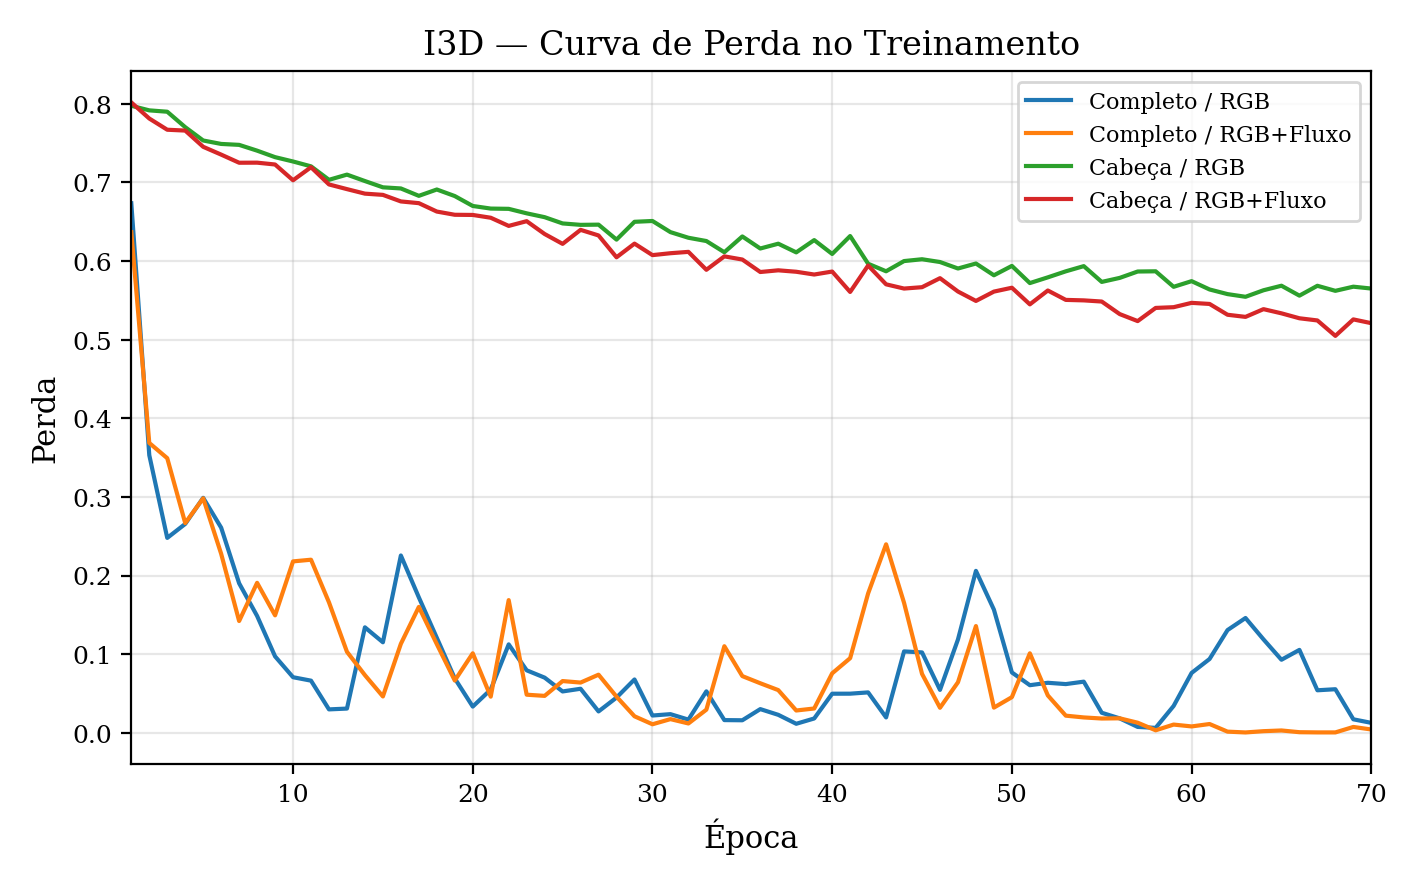
\includegraphics[height=0.25\textheight]{figuras/i3d_training_loss.png}
    
    {\footnotesize (a) I3D}
    
    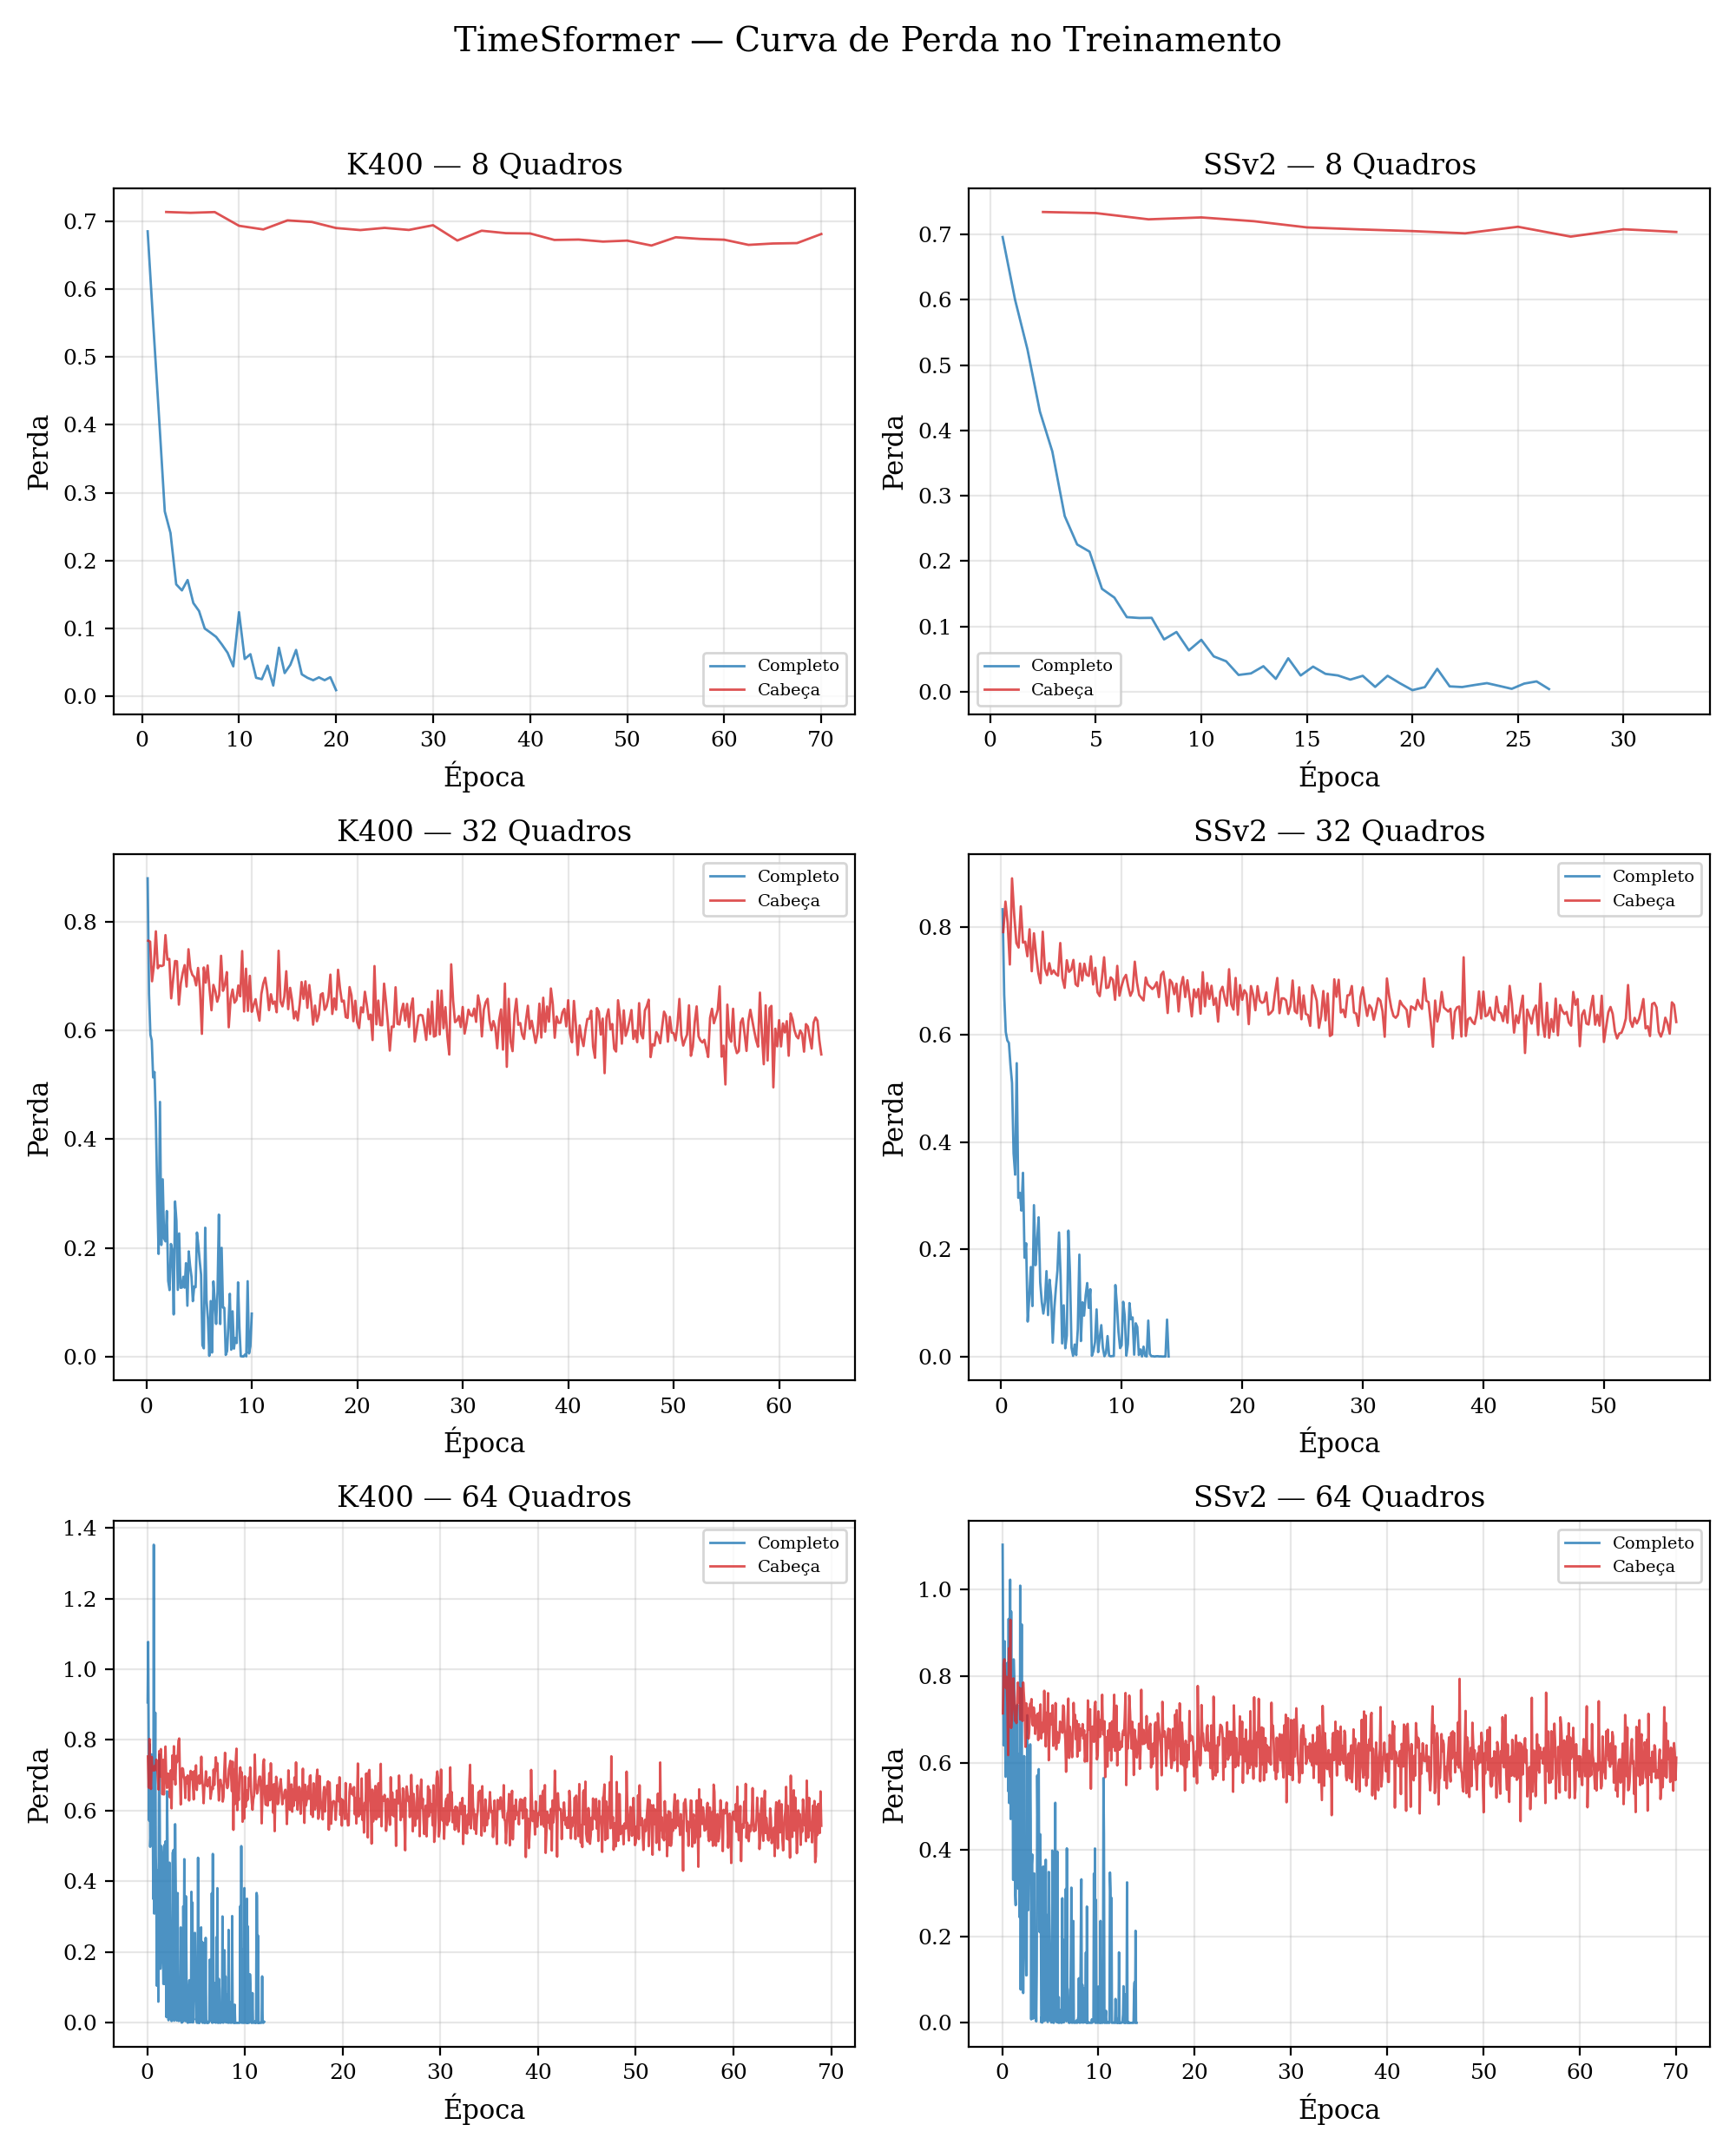
\includegraphics[height=0.65\textheight]{figuras/timesformer_training_loss.png}

    
    {\footnotesize (b) TimeSFormer}
    
    \legend{Fonte - Do autor.}
    \label{fig:training_loss}
\end{figure}


\section[Evolução das Métricas na Validação]{Evolução das Métricas na Validação}

O desempenho no conjunto de validação confirma as severas limitações impostas pelo treinamento somente da cabeça do modelo em comparação à atualização de todos os parâmetros. A \autoref{fig:i3d_val_metrics} ilustra a evolução da Acurácia, F1-Score e AUC-ROC para o modelo I3D. É evidente que as configurações de \textit{fine-tuning} completo convergem rapidamente logo nas primeiras épocas, superando a marca de 0,94 de AUC-ROC.

Um ponto de destaque é o comportamento do fluxo óptico: no cenário de \textit{fine-tuning} completo, a adição do fluxo não proporcionou ganhos significativos em relação à modalidade puramente RGB, sugerindo que a rede espacial atualizada consegue extrair os indícios de movimento necessários. No entanto, quando apenas a cabeça de classificação é treinada, a adição do fluxo óptico eleva visivelmente o desempenho, indicando que a explicitação do movimento compensa parcialmente a incapacidade da rede congelada de adaptar suas representações espaciais para a nova tarefa.

\begin{figure}[!htbp]
    \centering
    \caption[Evolução das métricas de validação para o I3D.]{Evolução das métricas de validação para o I3D.}
	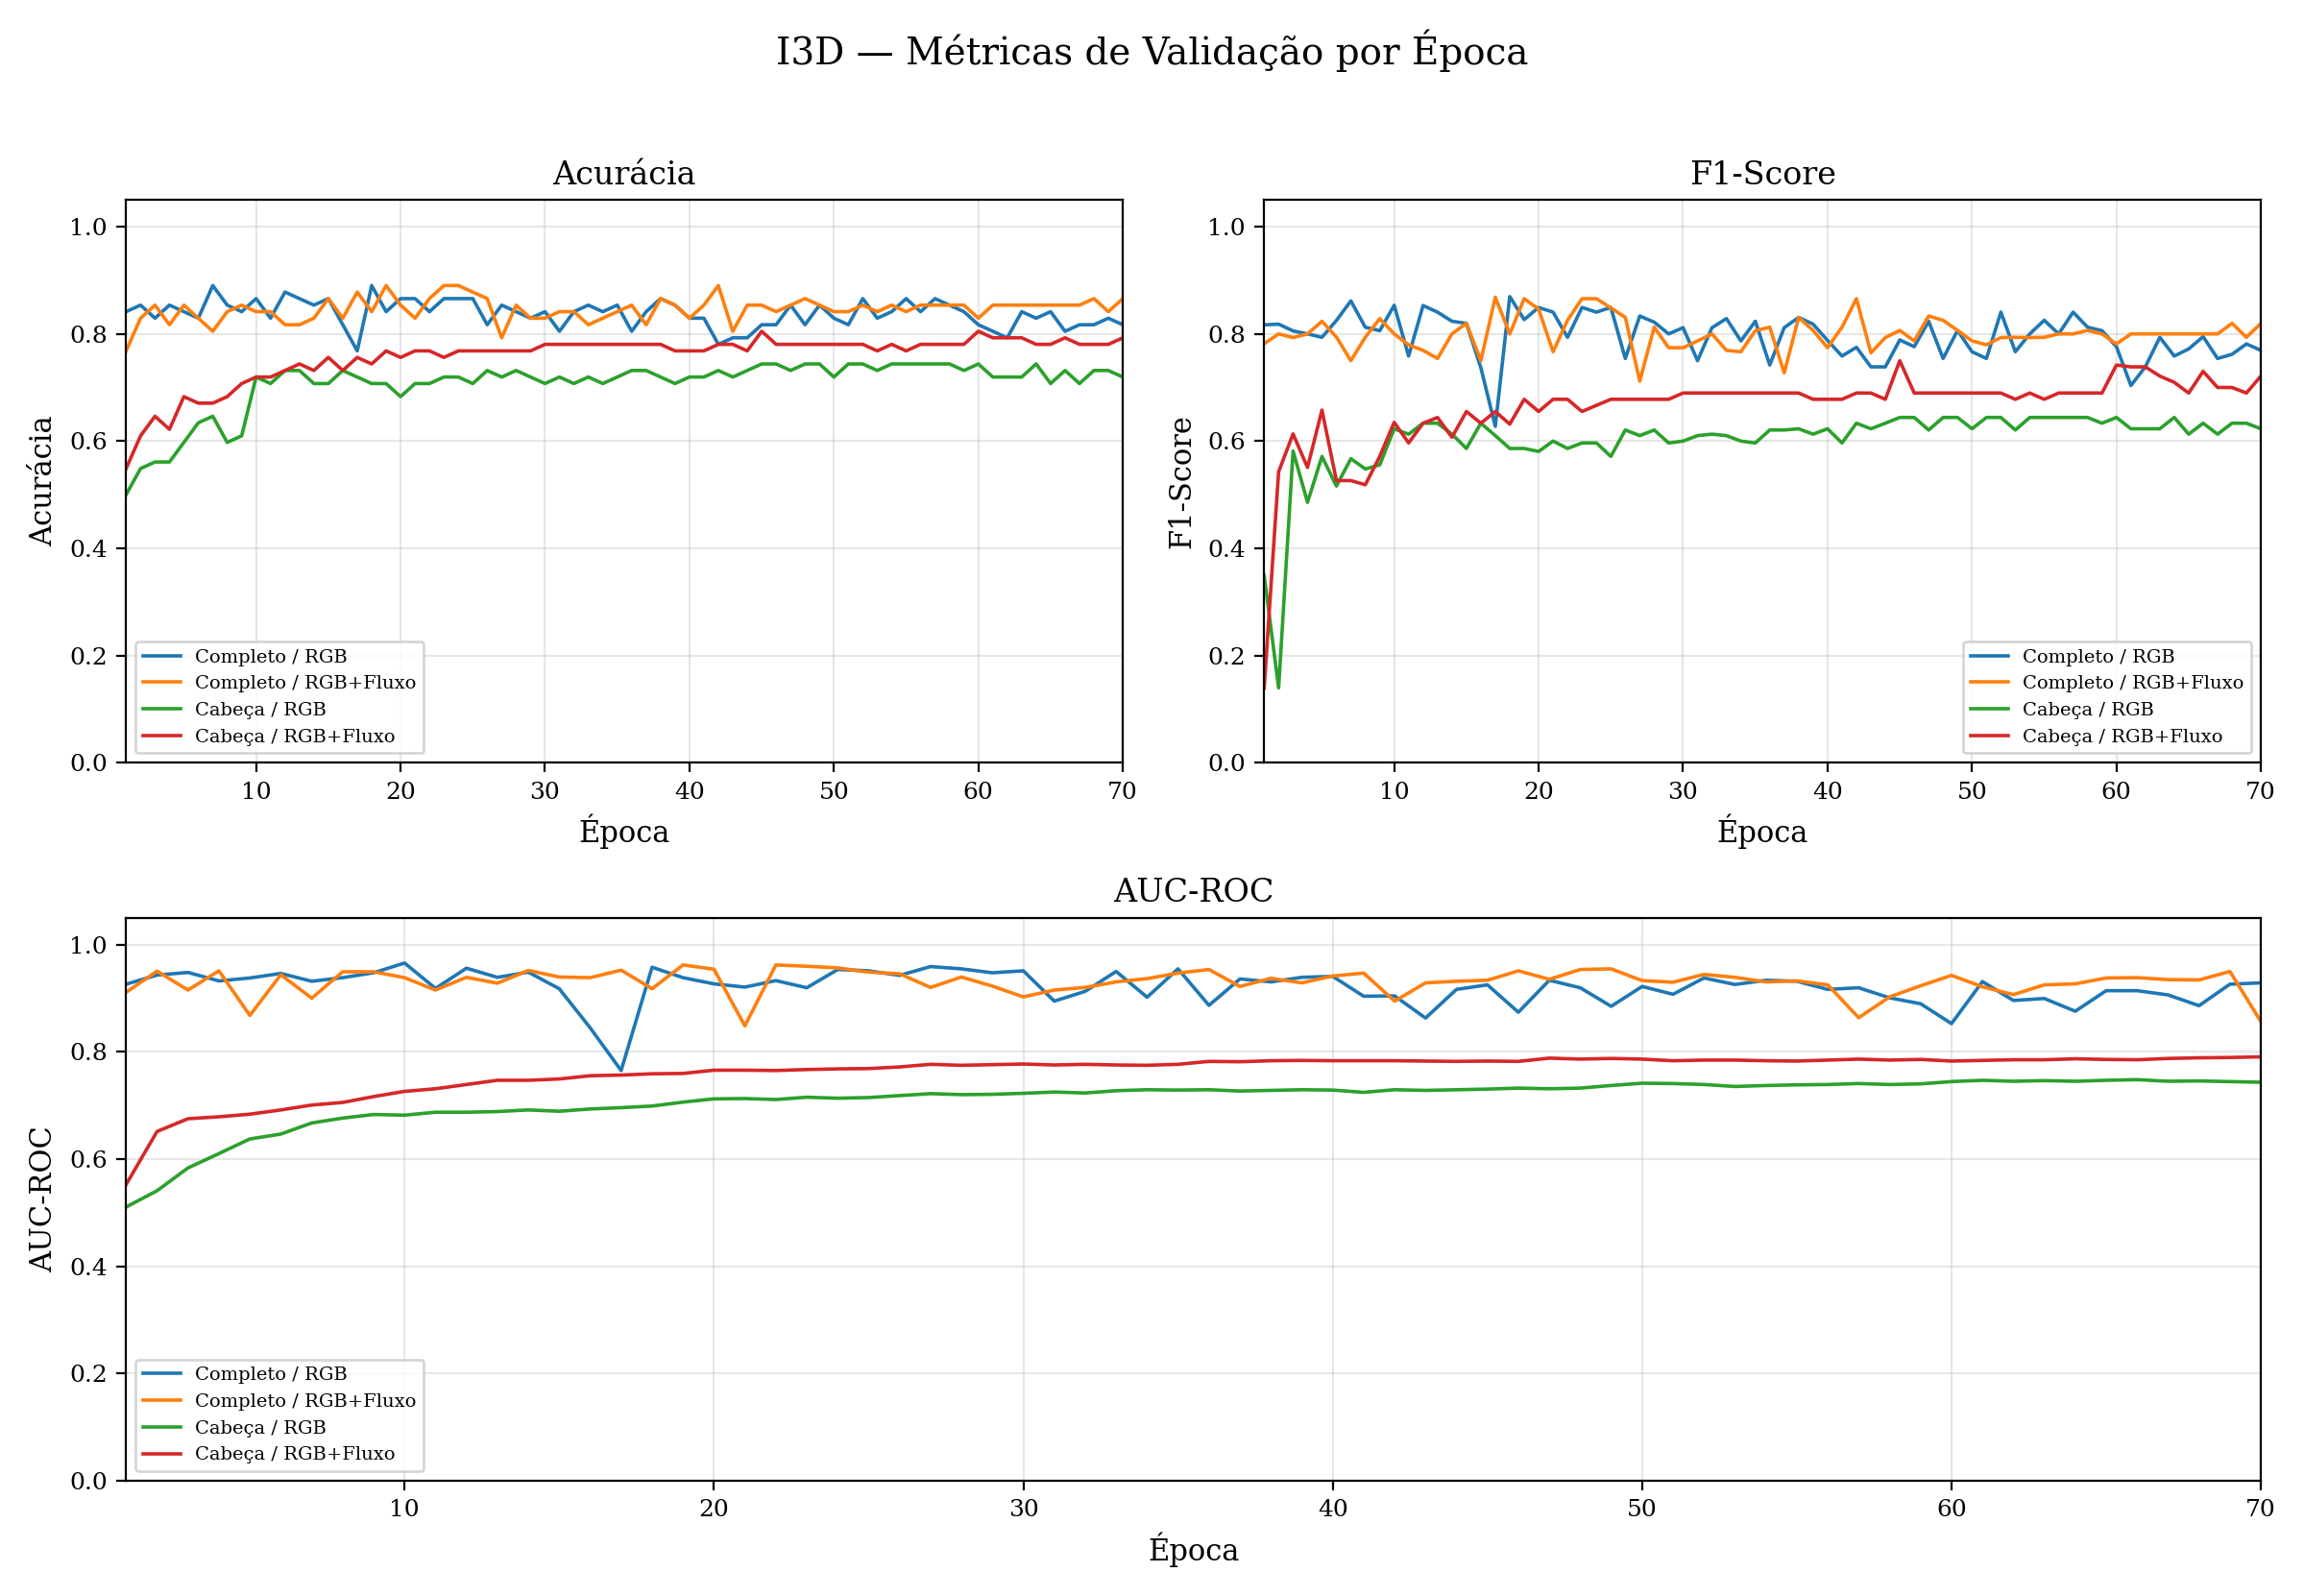
\includegraphics[width=\linewidth]{figuras/i3d_validation_metrics.png}
	\legend{Fonte - Do autor.}
    \label{fig:i3d_val_metrics}
\end{figure}

Para o TimeSFormer, as métricas de validação na \autoref{fig:timesformer_val_metrics} revelam uma disparidade ainda mais drástica entre as estratégias de treinamento. O treinamento exclusivo da cabeça de classificação falha em produzir resultados significativos, estagnando em valores baixos de Acurácia e F1-Score, demonstrando que o mecanismo de auto-atenção espaço-temporal requer forte adaptação ao novo domínio-alvo.

Em contrapartida, os modelos com \textit{fine-tuning} completo evidenciam grande robustez e eficiência, com os seis experimentos atingindo valores de AUC-ROC superiores a 0,91. Além da alta performance, nota-se que as configurações completas atingem a estabilidade de desempenho e acionam critérios de parada antecipada muito cedo, independentemente do banco de dados de pré-treino ou da resolução temporal de entrada (8, 32 ou 64 quadros). O aumento na quantidade de quadros não demonstrou alterar significativamente o teto máximo das métricas alcançadas, mas manteve a rápida convergência dos modelos.

\begin{figure}[htbp]
    \centering
    \caption[Evolução das métricas de validação para o TimeSFormer.]
    {Evolução das métricas de validação para o TimeSFormer.}
    
    \begin{minipage}{1\textwidth}
        \centering
        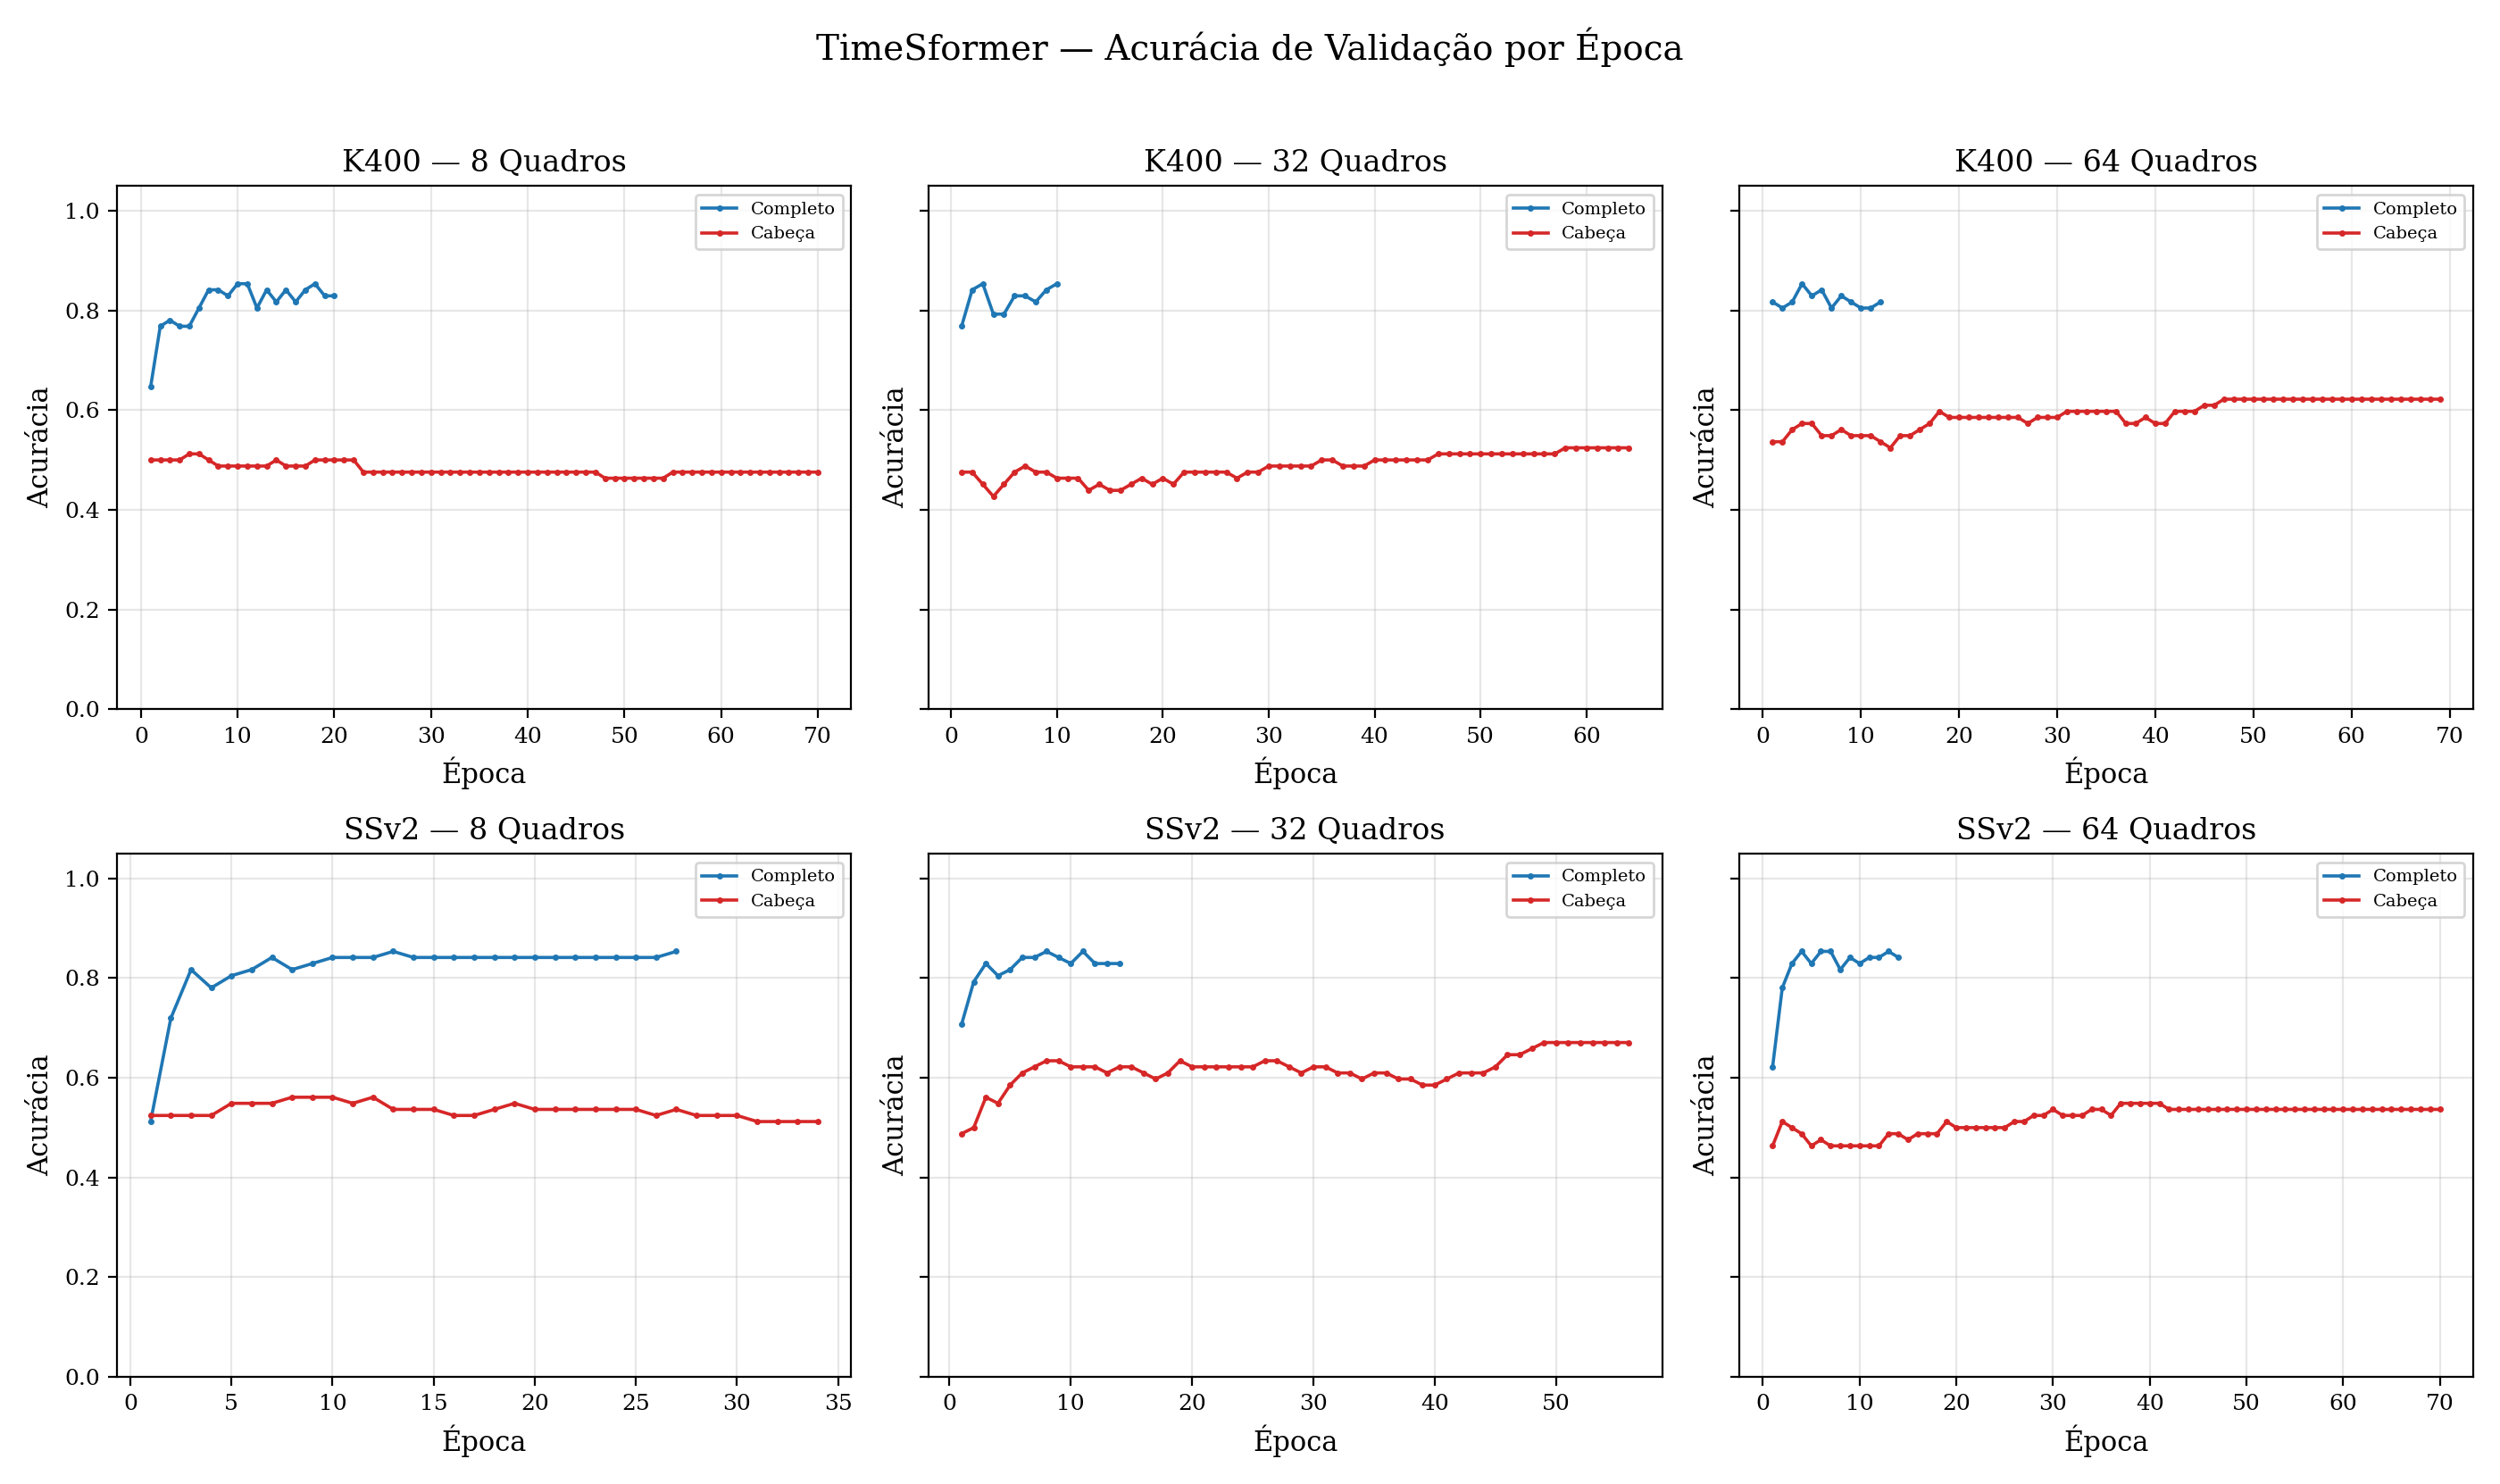
\includegraphics[height=0.31\textheight]{figuras/timesformer_val_eval_accuracy.png}
    \end{minipage}
    
    \begin{minipage}{1\textwidth}
        \centering
        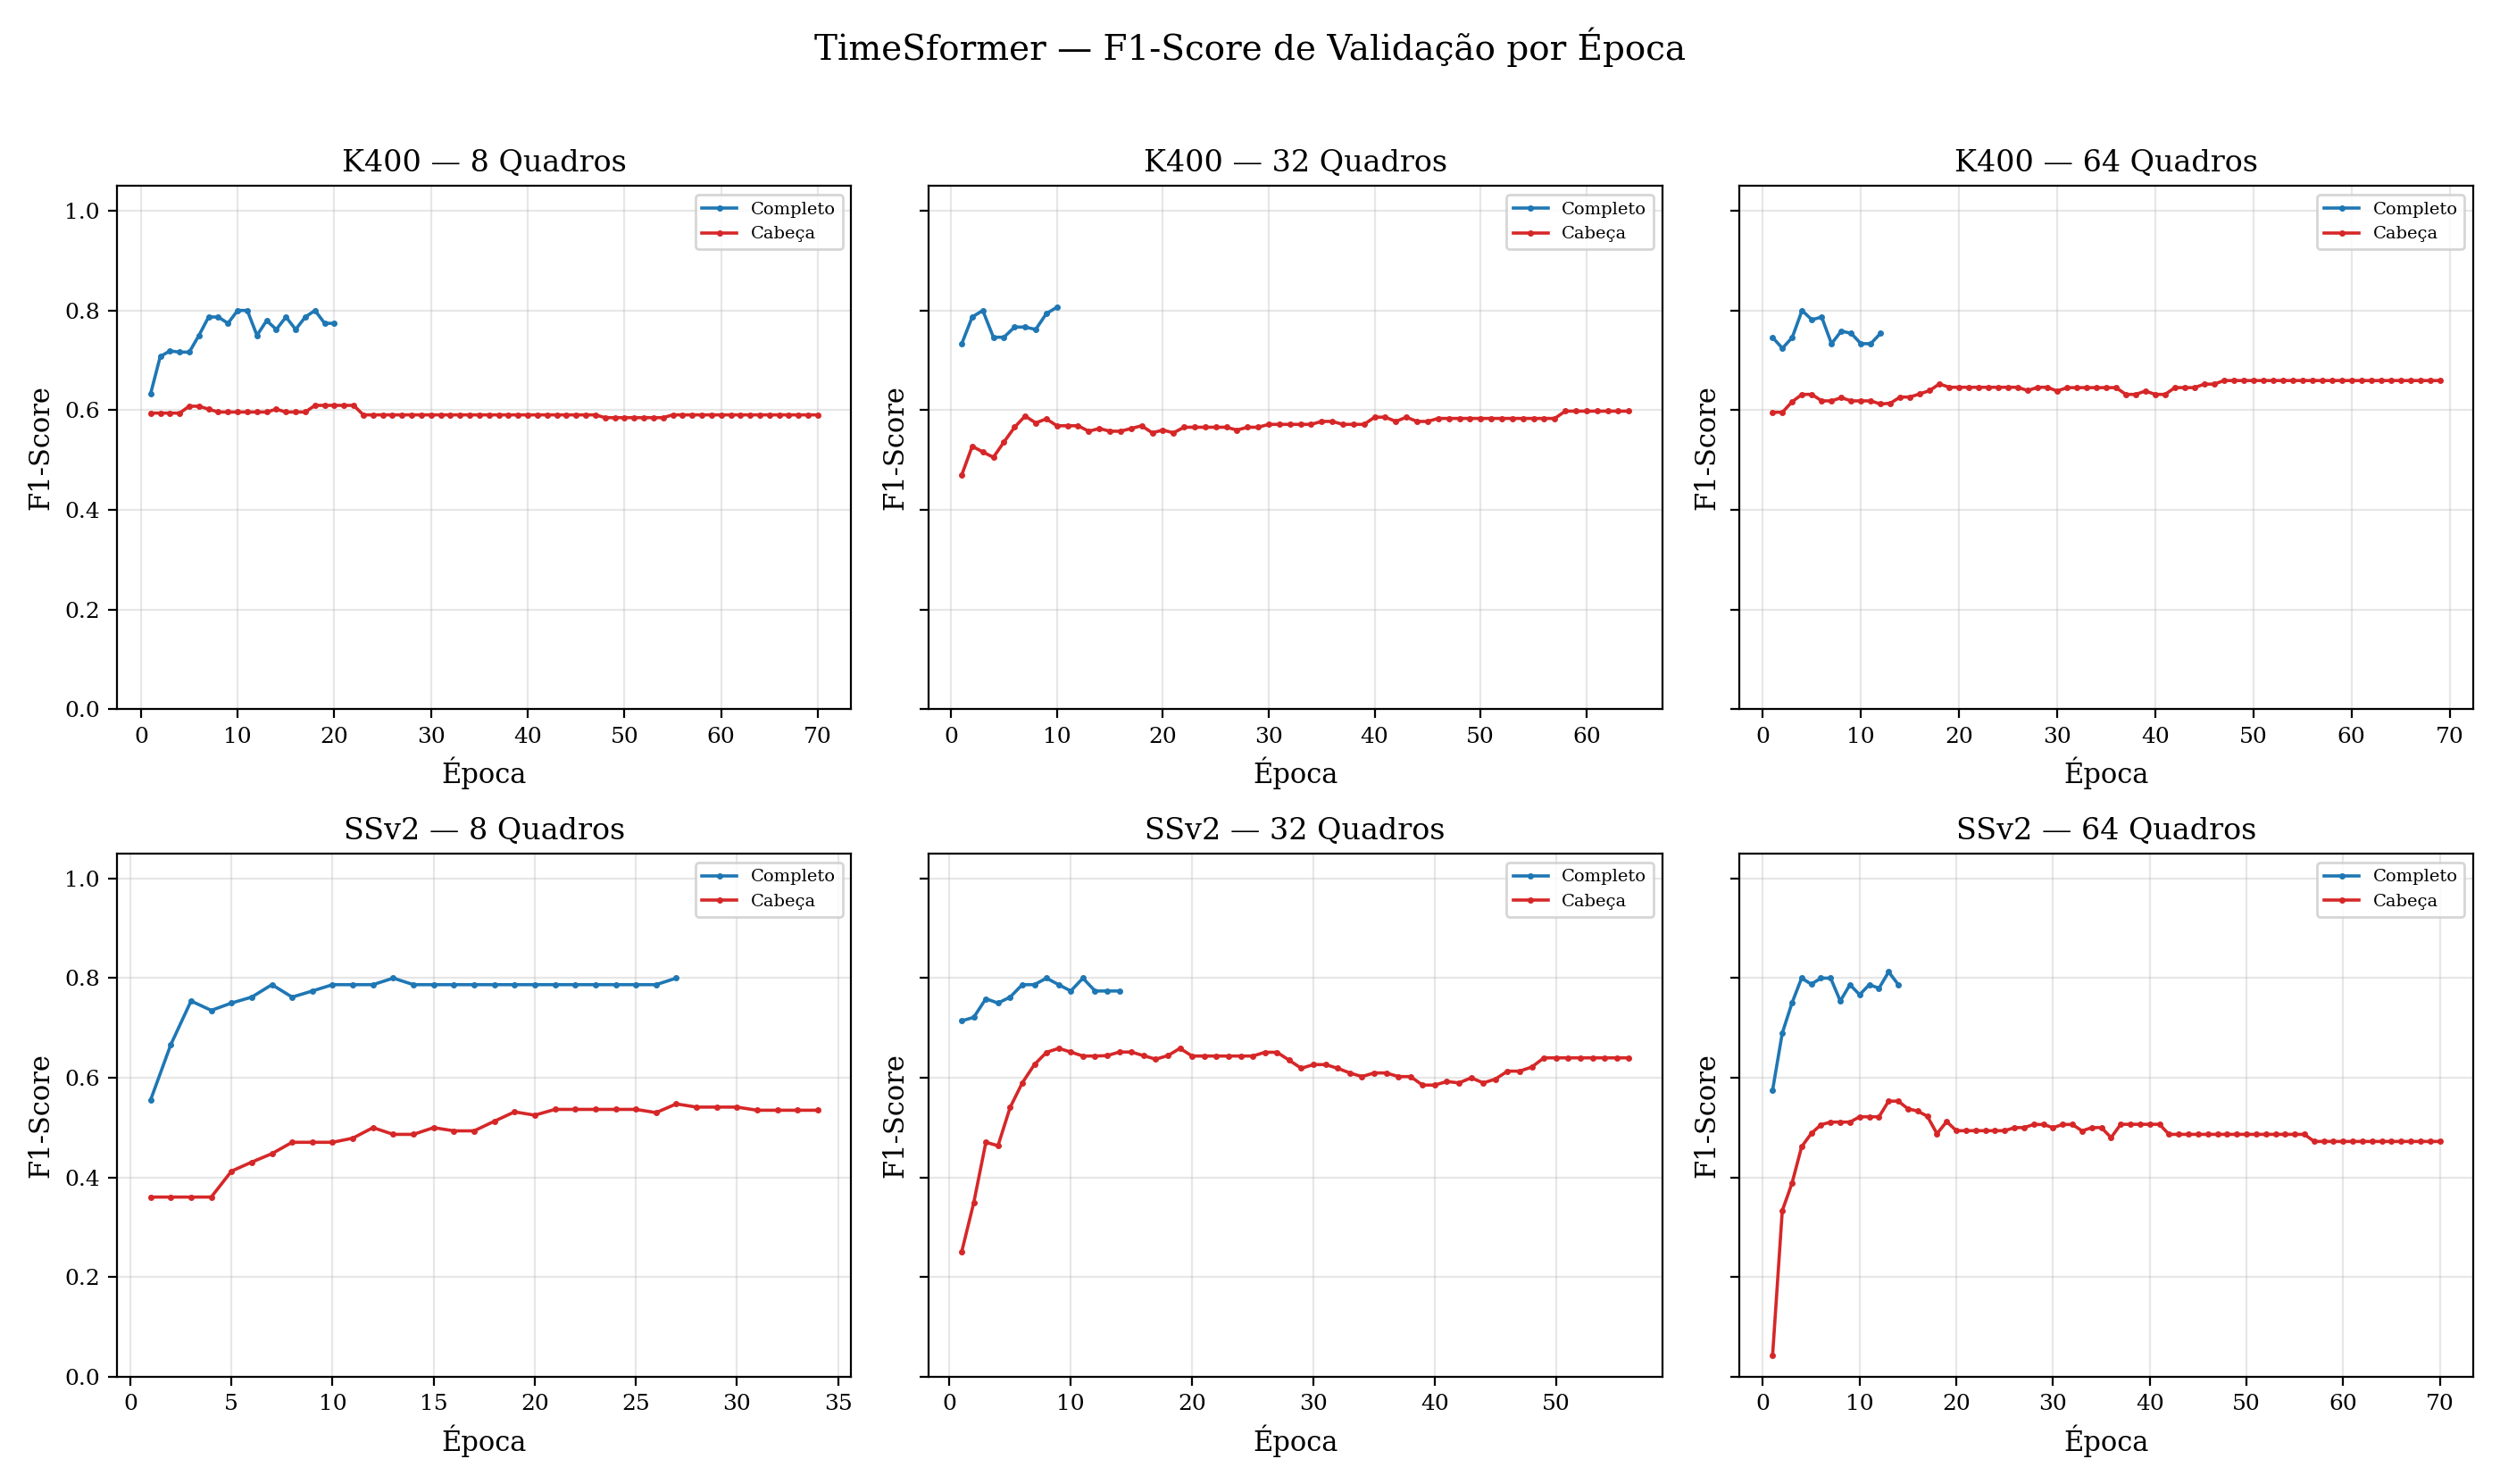
\includegraphics[height=0.31\textheight]{figuras/timesformer_val_eval_f1.png}
    \end{minipage}
    
    \begin{minipage}{1\textwidth}
        \centering
        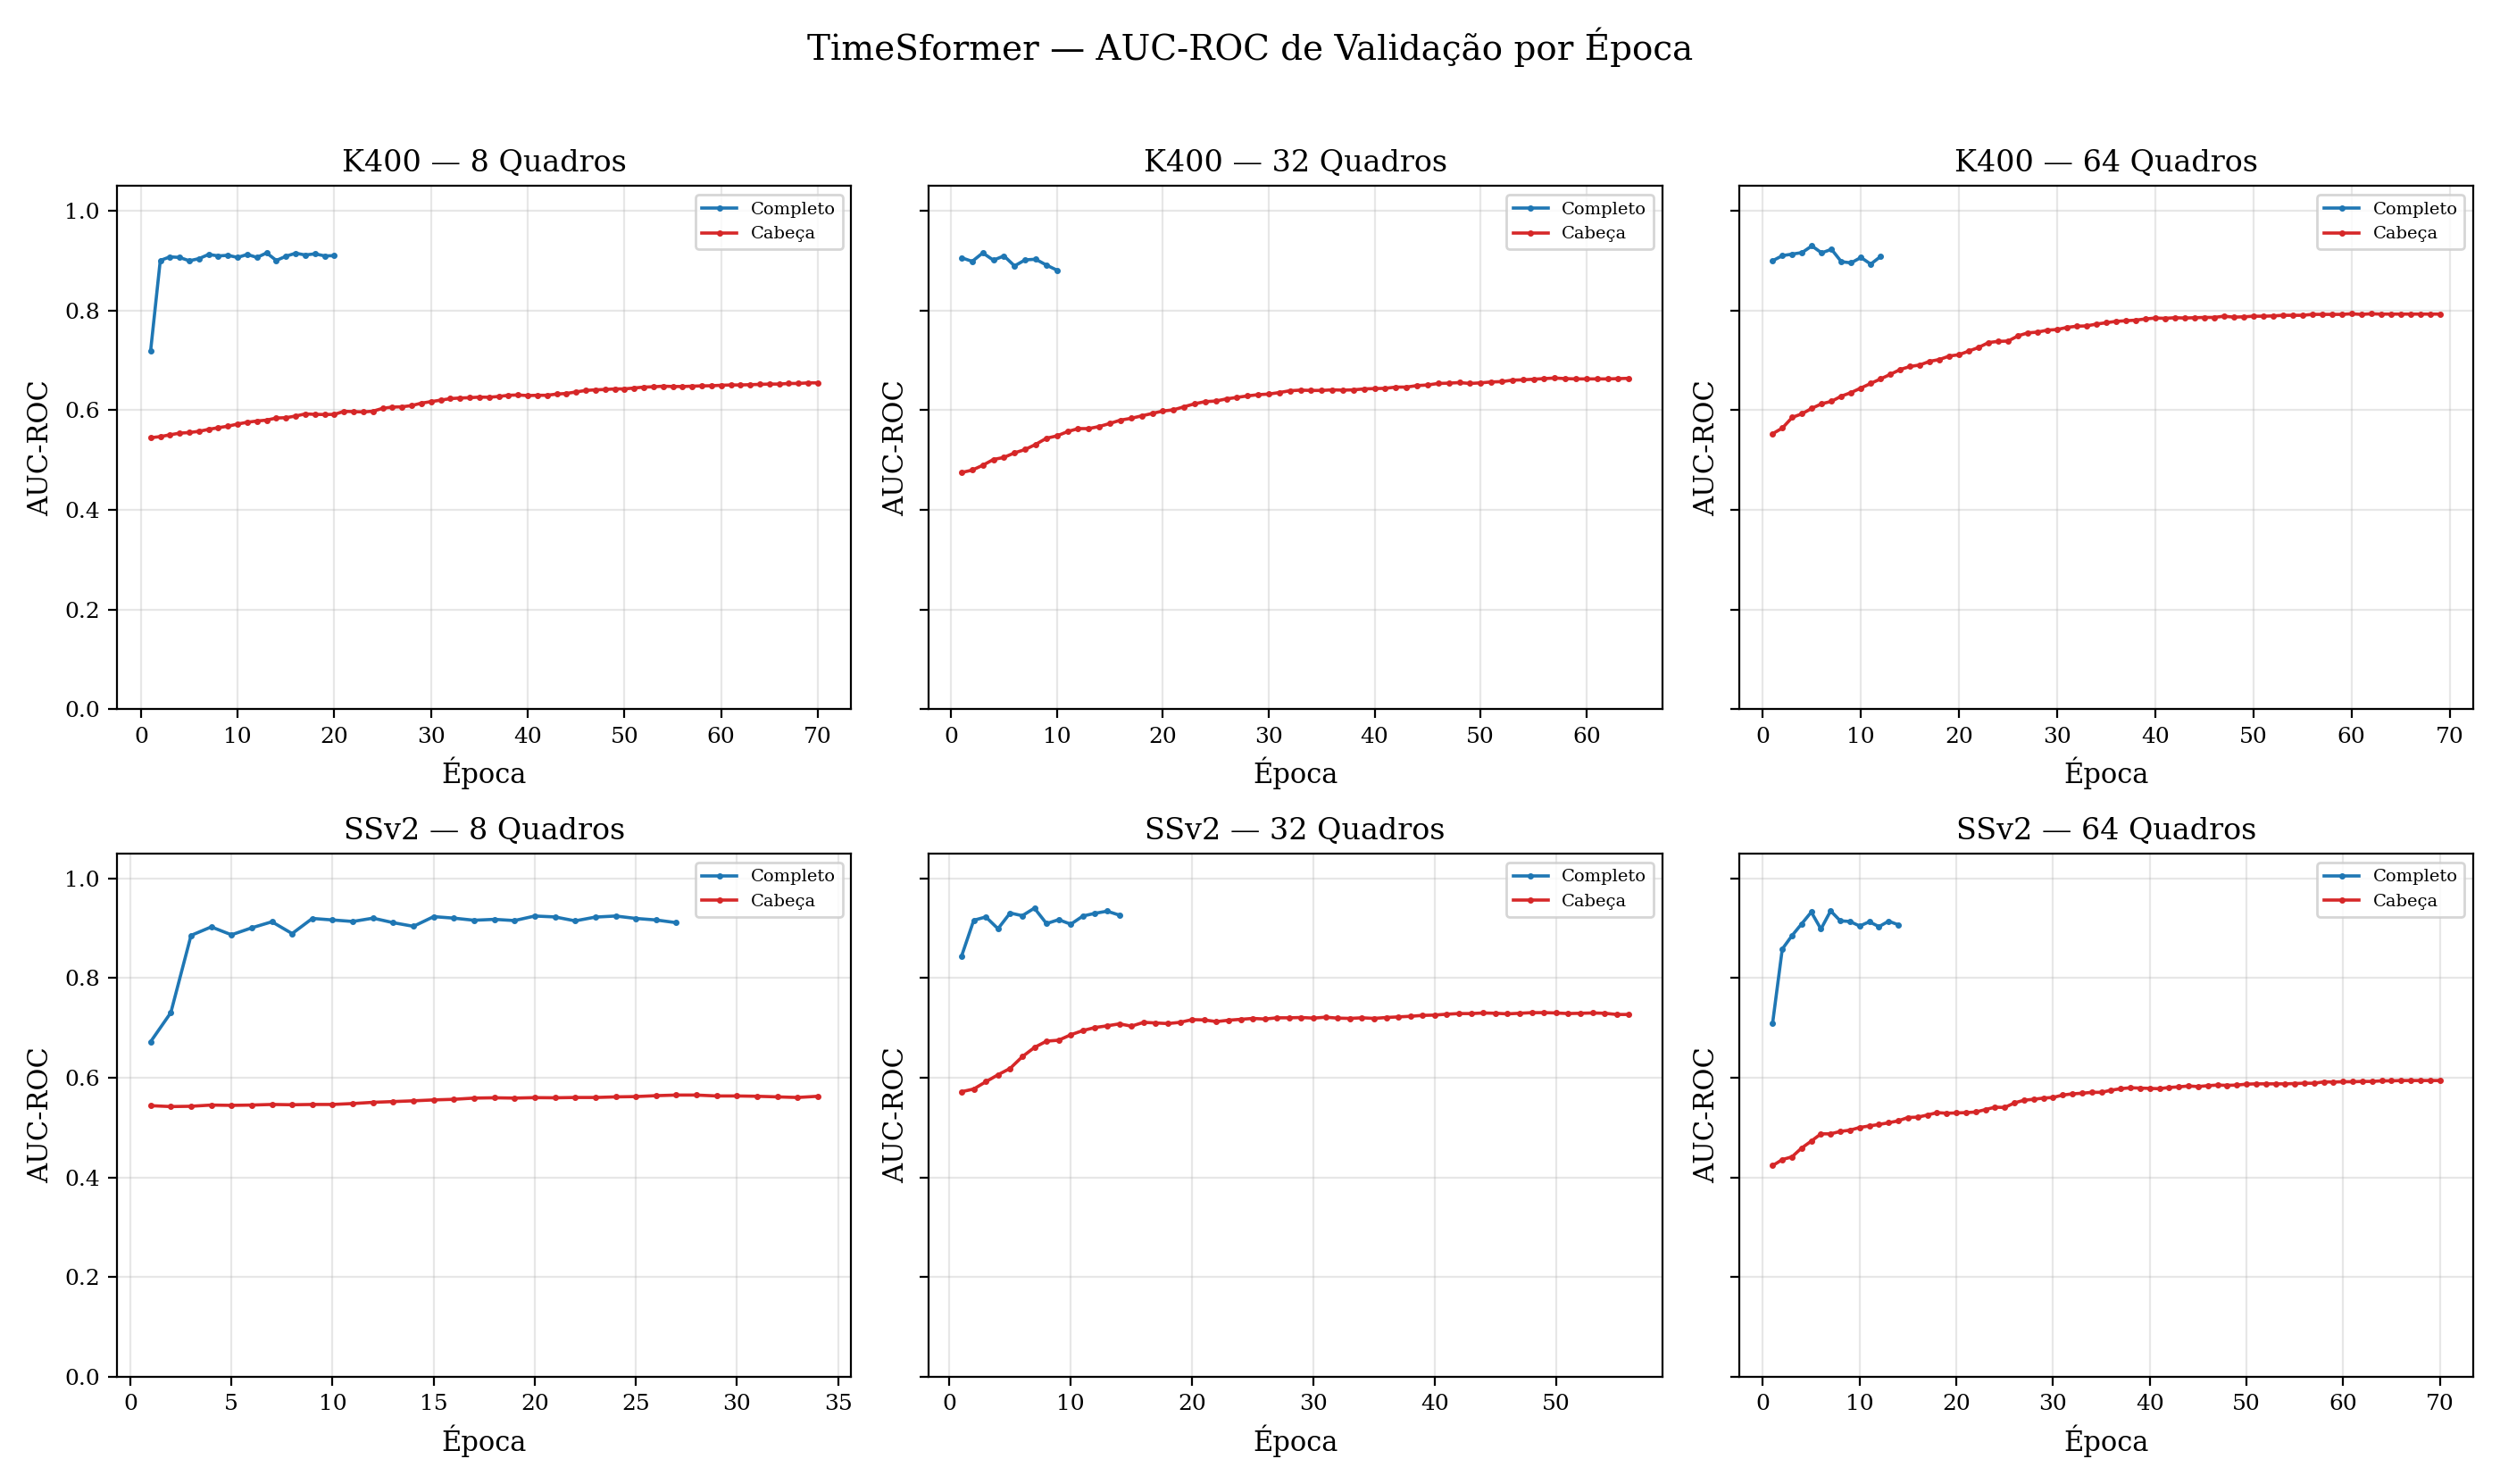
\includegraphics[height=0.31\textheight]{figuras/timesformer_val_eval_auc_roc.png}
    \end{minipage}

    \legend{Fonte - Do autor.}
    \label{fig:timesformer_val_metrics}
\end{figure}

\section[Avaliação Global e Seleção de Modelos]{Avaliação Global e Seleção de Modelos}

A fim de estabelecer o melhor representante de cada arquitetura, a \autoref{fig:auc_comparison_all} apresenta os resultados de AUC-ROC de validação para cada experimento. O modelo I3D na configuração Completa/RGB liderou esta etapa com AUC-ROC de 0,966, enquanto o TimeSFormer atingiu seu melhor desempenho na configuração pré-treinado no SSv2, com 32 quadros e ajuste completo, que obteve 0,940.

\begin{figure}[!htbp]
    \centering
    \caption[Comparação geral de AUC-ROC entre todas as 16 configurações experimentais.]{Comparação geral de AUC-ROC entre todas as 16 configurações experimentais.}
	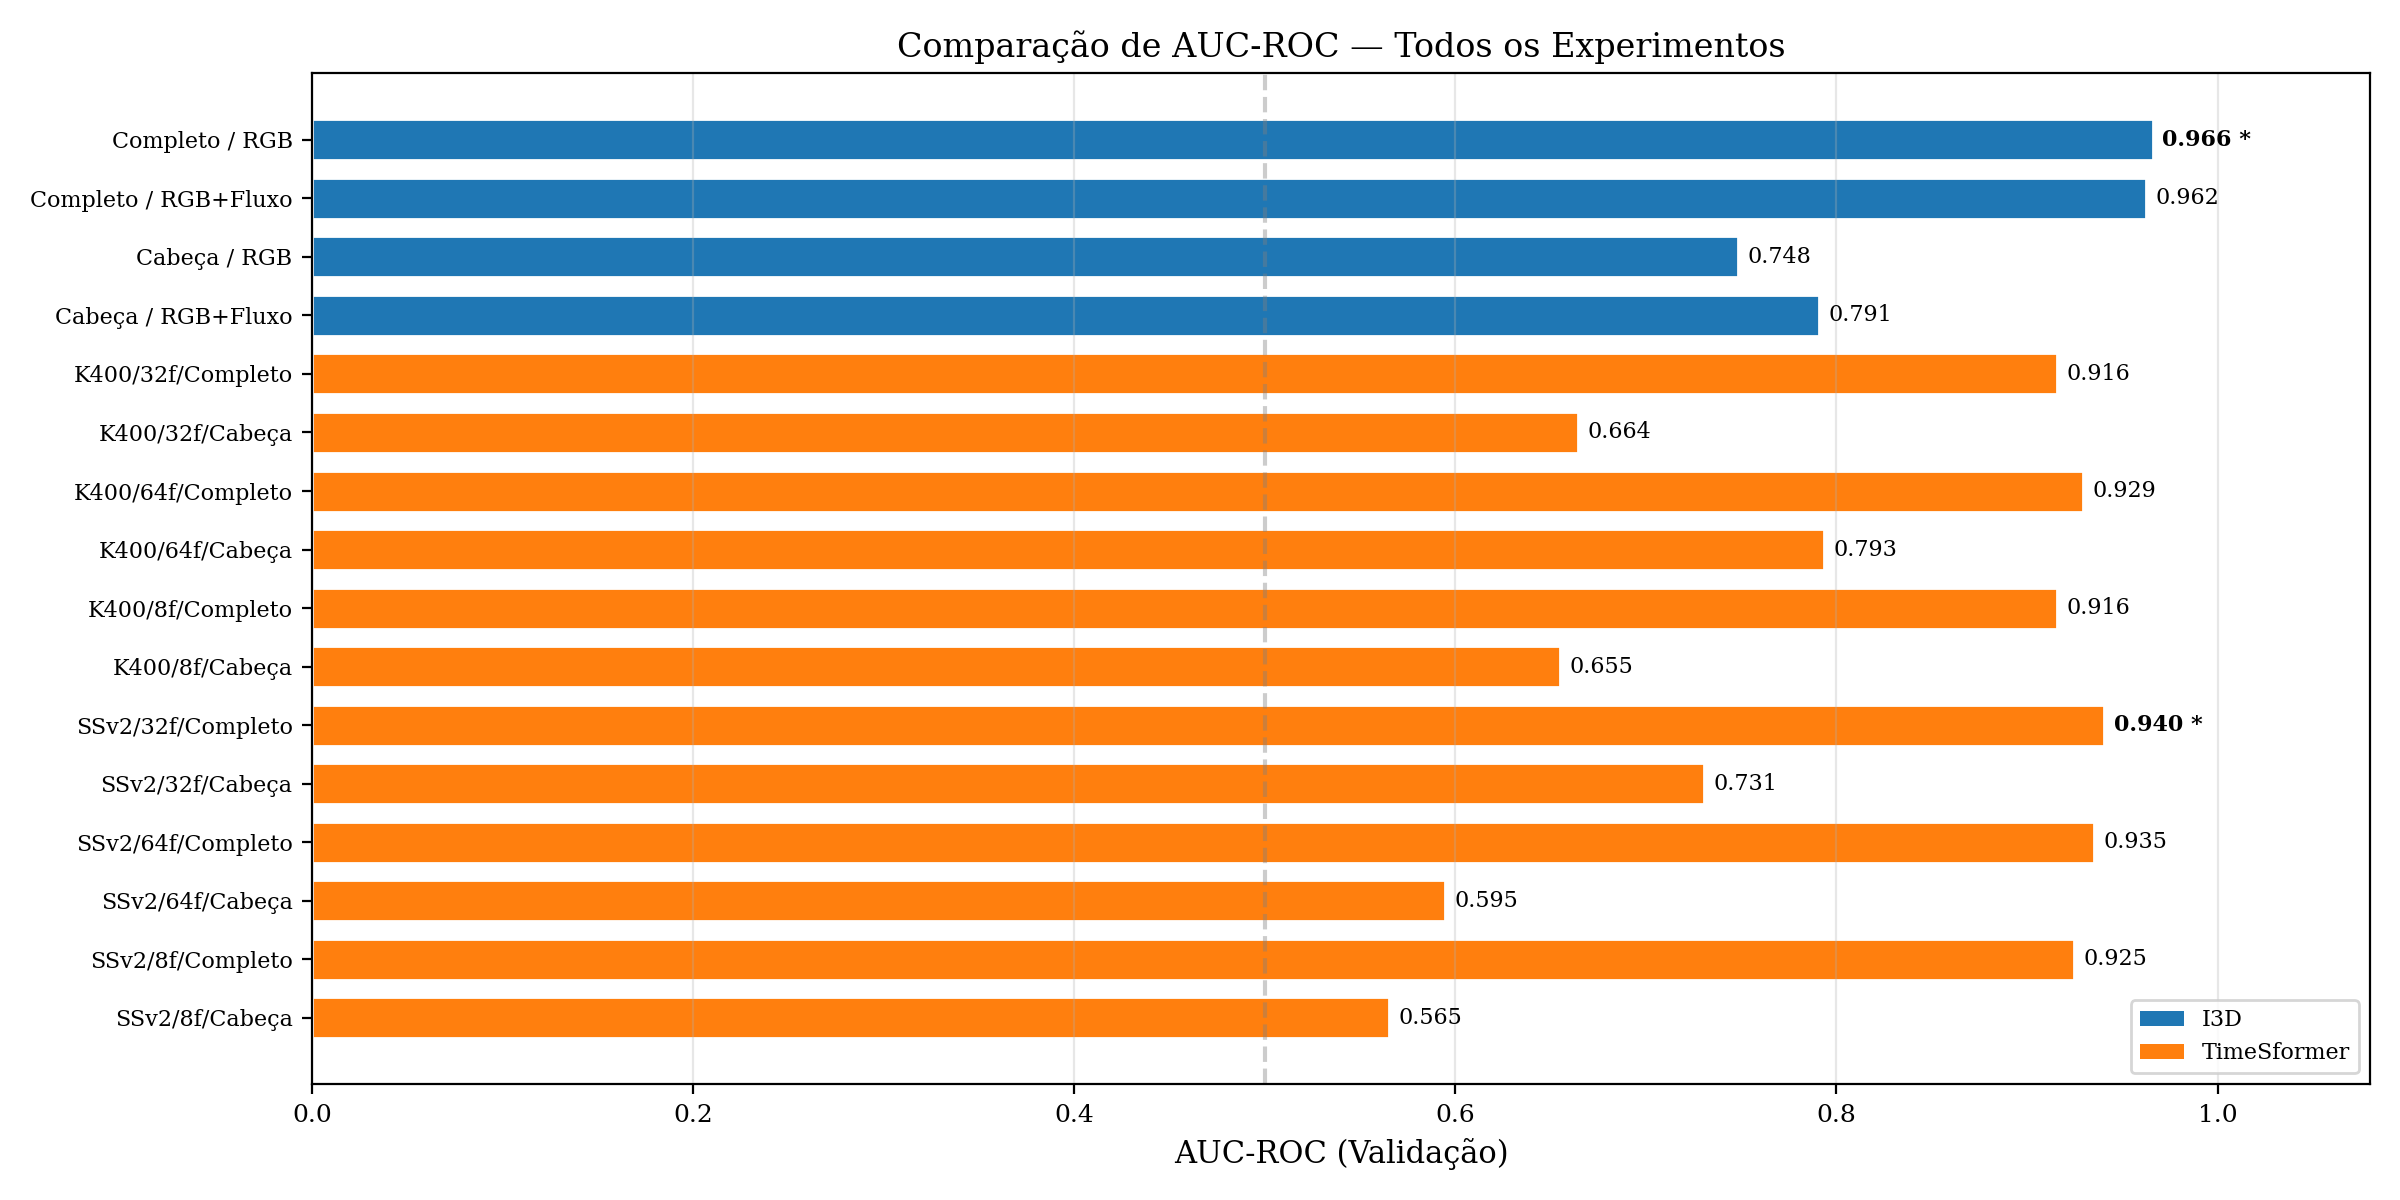
\includegraphics[width=1.0\textwidth]{figuras/auc_comparison_all.png}
	\legend{Fonte - Do autor.}
    \label{fig:auc_comparison_all}
\end{figure}


\section[Desempenho no Conjunto de Teste]{Desempenho no Conjunto de Teste}

A avaliação definitiva foi conduzida através da inferência com o melhor modelo de cada arquitetura no conjunto de teste composto por 83 amostras inéditas (47 da classe \textit{Normal} e 36 da classe \textit{Shoplifting}). Os resultados reportados na \autoref{tab:test_metrics} demonstram uma inversão no ranqueamento de desempenho em relação à fase de validação. Embora a avaliação do domínio priorize a revocação por meio do F2-Score, destaca-se que o modelo TimeSFormer (SSv2 / 32 quadros / Completo) também alcançou uma precisão de 100\%, evidenciando maior especificidade e um controle sobre os falsos positivos. Em contraste, o I3D (Completo / RGB) apresentou precisão de 72,3\%, indicando um viés mais conservador na tomada de decisão, com maior tendência a classificar amostras normais como casos anômalos. Já a diferença em revocação entre os modelos foi consideravelmente menor, de apenas 2,7\%, o que levou o TimeSFormer ao melhor resultado geral na avaliação final.

\begin{table}[htbp]
\centering
\caption{Métricas no conjunto de teste dos melhores modelos (Precisão, Revocação e F2-Score).}
\label{tab:test_metrics}
\resizebox{\textwidth}{!}{%
\begin{tabular}{lllll}
\toprule
Modelo & Experimento & Precisão & Revocação & F2-Score \\
\midrule
I3D & Completo / RGB & 0,723 & 0,944 & 0,890 \\
TimeSFormer & SSv2/32f/Completo & 1,000 & 0,917 & \textbf{0,932} \\
\bottomrule
\end{tabular}
}
\end{table}

As matrizes de confusão na \autoref{fig:test_confusion} detalham quantitativamente as classificações incorretas. A discrepância sugere que o I3D, além de conservador, pode ter sofrido um leve sobreajuste no conjunto de validação, enquanto o TimeSFormer demonstrou uma capacidade superior de generalização para dados totalmente desconhecidos. Esse comportamento deve-se, muito provavelmente, à superioridade arquitetural do mecanismo de auto-atenção na captura de dependências espaço-temporais globais e à robustez das representações obtidas durante o pré-treinamento, fatores que mitigam o risco de sobreajuste mesmo em um modelo com maior número de parâmetros.

\begin{figure}[!htbp]
    \centering
    \caption[Matrizes de confusão do melhor I3D e do melhor TimeSFormer no conjunto de teste.]{Matrizes de confusão do melhor I3D e do melhor TimeSFormer no conjunto de teste.}
	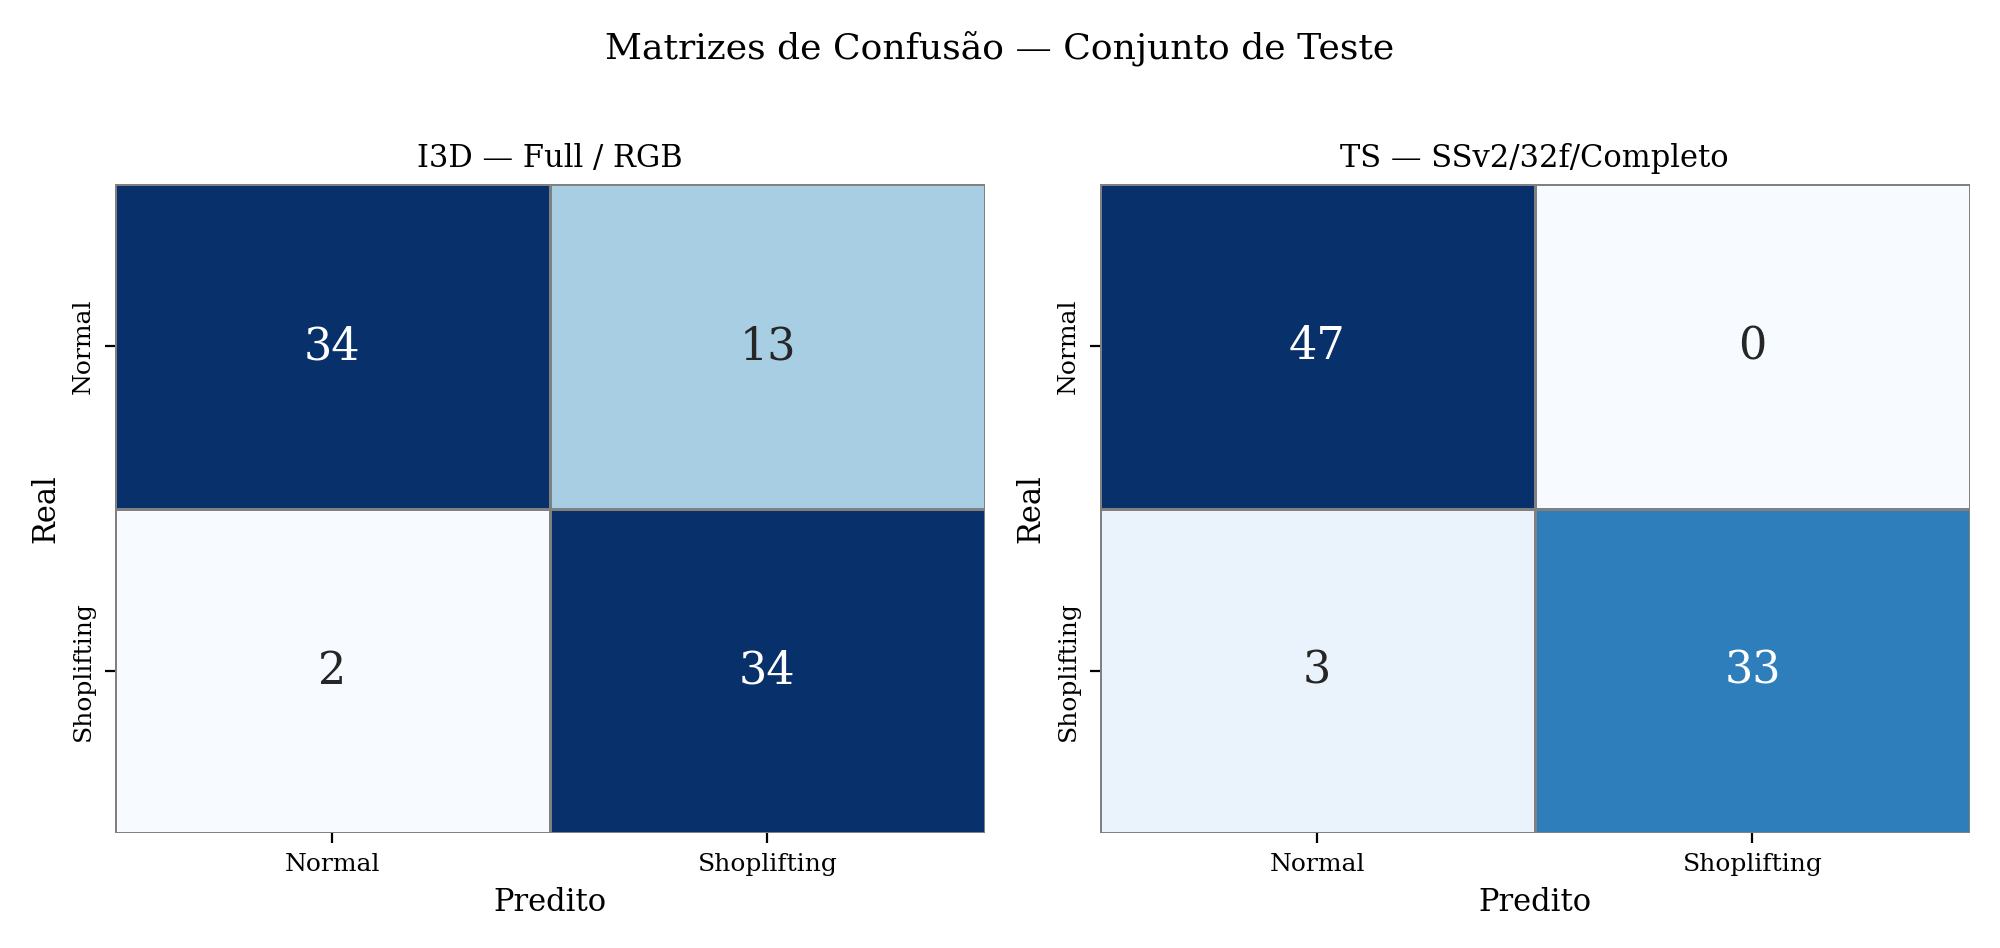
\includegraphics[width=0.9\textwidth]{figuras/test_confusion_matrices.png}
	\legend{Fonte - Do autor.}
    \label{fig:test_confusion}
\end{figure}

\section[Eficiência]{Eficiência}

Além do desempenho preditivo, os experimentos foram avaliados sob o viés da viabilidade prática considerando o tempo de inferência. A \autoref{tab:throughput} apresenta a taxa de transferência (\textit{throughput}) e o tempo de execução (\textit{runtime}) para uma configuração realista de implementação com uma GTX 1660 Super, utilizando lote unitário e entradas sintéticas aleatórias, de modo a evitar otimizações específicas de \textit{cache} ou carregamento de dados.

\begin{table}[htbp]
\centering
\caption{\textit{Throughput} de inferência dos melhores modelos I3D e TimeSFormer.}
\label{tab:throughput}
\resizebox{\textwidth}{!}{%
\begin{tabular}{llrr}
\toprule
Experimento & Amostras/s & ms/amostra \\
\midrule
I3D - Completo / RGB (64 quadros) & 12,57 & 79,53 \\
TimeSFormer - SSv2/32f/Completo (32 quadros) & 1,35 & 738,53 \\
\bottomrule
\end{tabular}
}
\end{table}

Em um cenário real de monitoramento, o processamento tende a ocorrer sobre fluxos contínuos de vídeo por meio de janelas temporais deslizantes, nas quais sequências consecutivas de quadros são periodicamente encaminhadas ao modelo. Dessa forma, a análise não depende de clipes previamente segmentados, permitindo que eventos mais longos sejam observados em múltiplas inferências sucessivas ao longo do tempo.

Nessa perspectiva, o modelo I3D apresentou um tempo de 79,53 ms por janela de 64 quadros. O baixo tempo de processamento oferece ampla margem para reduzir o passo entre janelas consecutivas, aumentar a frequência de atualização das predições e escalar a solução para múltiplas câmeras em uma mesma GPU. Tais características tornam a arquitetura particularmente atrativa em ambientes com restrições computacionais ou com demanda por menor latência operacional. O TimeSFormer, por sua vez, alcançou 738,53 ms por janela de 32 quadros. Embora apresente maior custo computacional, o tempo de inferência permanece compatível com aplicações em tempo real para fluxos individuais, especialmente quando associado a estratégias adequadas de amostragem temporal e infraestrutura dimensionada para essa finalidade.

Em termos práticos, os resultados indicam que ambas as arquiteturas são tecnicamente viáveis para sistemas de monitoramento contínuo, porém com compromissos distintos entre desempenho computacional e capacidade de implantação. O I3D destaca-se pela eficiência e escalabilidade, enquanto o TimeSFormer configura uma alternativa promissora em contextos nos quais maior disponibilidade de recursos computacionais permita explorar seu potencial de modelagem espaço-temporal.

\section[Síntese dos Resultados]{Síntese dos Resultados}

A condução e análise empírica dos 16 experimentos permite consolidar as seguintes constatações a respeito do reconhecimento de ações de furto nas condições avaliadas:

\begin{enumerate}
    \item \textbf{O ajuste profundo da rede foi essencial:} Apenas o treinamento com atualização integral dos pesos permitiu que os modelos aprendessem adequadamente a tarefa proposta. Em ambos os casos, limitar o treinamento à camada classificadora impediu convergência satisfatória.
    \item \textbf{A contribuição do fluxo óptico no I3D foi condicionada à estratégia de treino:} Quando houve a atualização integral dos pesos, o uso exclusivo de quadros RGB mostrou-se suficiente, tornando a inclusão do fluxo redundante. No entanto, ao congelar o extrator de características, fornecer o fluxo óptico foi fundamental para elevar o desempenho, compensando a incapacidade da rede rígida de extrair novos padrões de movimento apenas pela aparência visual.
    \item \textbf{O TimeSFormer demonstrou robustez:} Mesmo sob variações no número de quadros e no conjunto de pré-treino utilizado, o modelo sustentou métricas elevadas de AUC-ROC ao longo dos experimentos com treinamento completo.
    \item \textbf{Nos dados inéditos, o Transformer se destacou:} No conjunto de teste, o TimeSFormer alcançou a melhor capacidade de generalização, obtendo 100\% de precisão e o maior F2-Score, enquanto o I3D apresentou comportamento mais conservador, com maior ocorrência de falsos positivos.
    \item\textbf{Precisão adicional exige maior investimento computacional:} Observou-se uma troca direta entre custo e desempenho: o I3D se destacou pela rapidez e eficiência de inferência, ao passo que o TimeSFormer entregou resultados superiores em precisão e redução de alarmes falsos, porém com maior tempo de processamento.
\end{enumerate}

%TCC:


\chapter[Avaliação em Vídeos Reais]{Avaliação em Vídeos Reais}
%TCC:

\chapter[Conclusões]{Conclusões}
%TCC:

% \begin{figure}[!ht]
%     \centering
% 	\includegraphics[width=0.55\linewidth]{imagemExemplo.pdf}
% 	\caption[Isso é o que aparece no sumário]{Imagem de exemplo.}
% 	\label{fig:graficosVariandoTamanhoRede}
% \end{figure}


%TCC:
%TCC:
%TCC:
%TCC:





% ----------------------------------------------------------
% ELEMENTOS PÓS-TEXTUAIS
% ----------------------------------------------------------
\postextual


% ----------------------------------------------------------
% Referências bibliográficas
% ----------------------------------------------------------
\bibliography{abntex2-modelo-references}


%% ----------------------------------------------------------
%% Apêndices TCC: só mantenha se for pertinente.
%% ----------------------------------------------------------

% ---
% Inicia os apêndices
% ---
% \begin{apendicesenv}

% Imprime uma página indicando o início dos apêndices
% \partapendices

% % ----------------------------------------------------------
% \chapter{Quisque libero justo}
% % ----------------------------------------------------------

% \lipsum[50]

% % ----------------------------------------------------------
% \chapter{Coisas que fiz e que achei interessante mas não tanto para entrar no corpo do texto}
% % ----------------------------------------------------------
% \lipsum[55-57]

% \end{apendicesenv}
% % ---


% % ----------------------------------------------------------
% % Anexos %TCC: so mantenha se pertinente.
% % ----------------------------------------------------------

% % ---
% % Inicia os anexos
% % ---
% \begin{anexosenv}

% % Imprime uma página indicando o início dos anexos
% \partanexos

% % ---
% \chapter{Eu sempre quis aprender latim}
% % ---
% \lipsum[30]

% % ---
% \chapter{Coisas que eu não fiz mas que achei interessante o suficiente para colocar aqui}
% % ---

% \lipsum[31]

% % ---
% \chapter{Fusce facilisis lacinia dui}
% % ---

% \lipsum[32]

% \end{anexosenv}

%---------------------------------------------------------------------
% INDICE REMISSIVO
%---------------------------------------------------------------------

\printindex



\end{document}